%%%%%%%%%%%%%%%%%%%%%%%%%%%%%%%%%%%%%%%%%%%%%%%%%%%%%%%%%%%%%%%%%%%%%%%%%%%%%
%%%
%%% File: thesis.tex, version 1.9, May 2016
%%%
%%% =============================================
%%% This file contains a template that can be used with the package
%%% cs.sty and LaTeX2e to produce a thesis that meets the requirements
%%% of the Computer Science Department from the Technical University of Cluj-Napoca
%%%%%%%%%%%%%%%%%%%%%%%%%%%%%%%%%%%%%%%%%%%%%%%%%%%%%%%%%%%%%%%%%%%%%%%%%%%%%

\documentclass[12pt,a4paper,twoside]{report}         
\usepackage{cs}   
\usepackage{times}
\usepackage{graphicx}
\usepackage{latexsym}
\usepackage{amsmath,amsbsy}
\usepackage{amssymb}
\usepackage[matrix,arrow]{xy}
\usepackage[T1]{fontenc}
\usepackage{ae,aecompl}
\usepackage{romanian} %definitii pentru diacritice; 
\usepackage{amstext}
\usepackage{graphics}
\usepackage[T1]{fontenc}
\usepackage{ae,aecompl}
\usepackage{algorithm}
%\usepackage{algorithmic}
\usepackage{color}
\usepackage{algpseudocode}
\usepackage{subcaption}
\usepackage{multicol}
\usepackage{hyperref}
\newcommand{\argmin}
{\operatornamewithlimits{argmin}}

% \mastersthesis
\diplomathesis
% \leftchapter
\centerchapter
% \rightchapter
\singlespace
% \oneandhalfspace
% \doublespace

\renewcommand{\thesisauthor}{Andreea TOMOIAG'A}    %% Your name.
\renewcommand{\thesismonth}{Iunie}     %% Your month of graduation.
\renewcommand{\thesisyear}{2018}      %% Your year of graduation.
\renewcommand{\thesistitle}{DETEC'TIA S'AGE'TILOR DIREC'TIONALE FOLOSIND RE'TELE CONVOLU'TIONALE} % Title
\renewcommand{\thesissupervisor}{Conf.Dr.Ing. Florin ONIGA}
\newcommand{\department}{FACULTATEA DE AUTOMATIC'A 'SI CALCULATOARE\\
DEPARTAMENTUL CALCULATOARE}
\newcommand{\thesis}{LUCRARE DE LICEN'T'A}
\newcommand{\uline}[1]{\rule[0pt]{#1}{0.4pt}}
%\renewcommand{\thesisdedication}{P'arin'tilor mei}
\newcommand{\utcnlogo}{\includegraphics[width=15cm]{img/utcn.jpg}}

\begin{document}
%\frontmatter
%\pagestyle{headings}

\newenvironment{definition}[1][Defini'tie.]{\begin{trivlist}
\item[\hskip \labelsep {\bfseries #1}]}{\end{trivlist}}



%\thesistitle                    %% Generate the title page.
%\authordeclarationpage                %% Generate the declaration page.

\pagenumbering{arabic}
\setcounter{page}{4}
\setcounter{tocdepth}{4}
\setcounter{secnumdepth}{4}


\begin{center}
%\includegraphics[width=15cm]{img/tucn.jpg}  
\utcnlogo

{\bf \department}

\vspace{4cm}

{\bf \thesistitle} %LICENSE THESIS TITLE}

\vspace{1.5cm}

\thesis

\vspace{6cm}

Absolvent: {\bf \thesisauthor} 

Conduc'ator 'stiin'tific: {\bf \thesissupervisor}

\vspace{2cm}
{\bf \thesisyear}
\end{center}

\thispagestyle{empty}
\newpage

\begin{center}
\utcnlogo

{\bf \department}
\end{center}
\vspace{0.5cm}

%\begin{small}
\begin{tabular}{p{7cm}p{8cm}}
 %\hspace{-1cm}& VIZAT,\\
 \hspace{-1cm}DECAN, & DIRECTOR DEPARTAMENT,\\
\hspace{-1cm}{\bf Prof. dr. ing. Liviu MICLEA} & {\bf Prof. dr. ing. Rodica POTOLEA}\\  
\end{tabular}
 
\vspace{2cm}

\begin{center}
Absolvent: {\bf \thesisauthor}

\vspace{1cm}

{\bf \thesistitle}
\end{center}

\vspace{1cm}

\begin{enumerate}
 \item {\bf Enun'tul temei:} {\it Scurt'a descriere a temei lucr'arii de licen't'a 'si datele ini'tiale}
\item {\bf Con'tinutul lucr'arii:} {\it (enumerarea p'ar'tilor componente) Exemplu: Pagina de prezentare, aprecierile coordonatorului de lucrare, titlul capitolului 1, titlul capitolului 2, titlul capitolului n, bibliografie, anexe.}
\item {\bf Locul document'arii:} {\it Exemplu}: Universitatea Tehnic'a din Cluj-Napoca, Departamentul Calculatoare
\item {\bf Consultan'ti:}
\item {\bf Data emiterii temei:} 1 Noiembrie 2016
\item {\bf Data pred'arii:} 21 Februarie 2018 {\it (se va completa data pred'arii)}
  \end{enumerate}
\vspace{1.2cm}

\hspace{6cm} Absolvent: \uline{6cm} 

\vspace{0.5cm}
\hspace{6cm} Coordonator 'stiin'tific: \uline{5cm} 
%\end{small}

\thispagestyle{empty}


$ $
%\begin{center}
%\utcnlogo

%{\bf \department}
%\end{center}

\thispagestyle{empty}
\newpage

\begin{center}
\utcnlogo

{\bf \department}
\end{center}

\vspace{0.5cm}

\begin{center}
{\bf
Declara'tie pe proprie r'aspundere privind\\ 
autenticitatea lucr'arii de licen't'a}
\end{center}
\vspace{1cm}



Subsemnatul(a) \\
\uline{14.8cm}, 
legitimat('a) cu \uline{4cm} seria \uline{3cm} nr. \uline{4cm}\\
CNP \uline{9cm}, autorul lucr'arii \uline{2.8cm}\\
\uline{16cm}\\
\uline{16cm}\\
elaborat'a 'in vederea sus'tinerii examenului de finalizare a studiilor de licen't'a la Facultatea de Automatic'a 'si Calculatoare, Specializarea \uline{7cm} din cadrul Universit'a'tii Tehnice din Cluj-Napoca, sesiunea \uline{4cm} a anului universitar \uline{3cm}, declar pe proprie r'aspundere, c'a aceast'a lucrare este rezultatul propriei activit'a'ti intelectuale, pe baza cercet'arilor mele 'si pe baza informa'tiilor ob'tinute din surse care au fost citate, 'in textul lucr'arii 'si 'in bibliografie.

Declar, c'a aceast'a lucrare nu con'tine por'tiuni plagiate, iar sursele bibliografice au fost folosite cu respectarea legisla'tiei rom\ia ne 'si a conven'tiilor interna'tionale privind drepturile de autor.

Declar, de asemenea, c'a aceast'a lucrare nu a mai fost prezentat'a 'in fa'ta unei alte comisii de examen de licen't'a.

'In cazul constat'arii ulterioare a unor declara'tii false, voi suporta sanc'tiunile administrative, respectiv, \emph{anularea examenului de licen't'a}.

\vspace{1.5cm}

Data \hspace{8cm} Nume, Prenume

\vspace{0.5cm}

\uline{3cm} \hspace{5cm} \uline{5cm}

\vspace{1cm}
\hspace{9.4cm}Semn'atura

\thispagestyle{empty}

\newpage


%\listoftables
%\listoffigures

%\clearpage 
%\newpage

%\begin{comment}
\include{guideline} 
%\end{comment}

\newpage

\tableofcontents
\newpage



\chapter{Introducere - Contextul proiectului}
\pagestyle{headings}
\setcounter{page}{1}
Dorin'ta 'si necesitatea zilnic'a de deplasare au f'acut ca industria autovehiculelor rutiere s'a creasc'a 'si s'a se dezvolte. De-a lungul anilor, num'arul 'soferilor 'si al autovehiculelor din mediul urban 'si rural a crescut exponen'tial, duc\^and la m'arirea aglomera'tiei 'si a blocajelor rutiere.  Totodat'a, a crescut 'si  num'arul de accidente produse din erori umane, fie ele din neglijen'ta acordat'a  drumului sau din cauza stilul de condus agresiv. 
 

\section{Contextul proiectului}
\subsection{Driver assistance}
\^In prezent, principalul interes al industriei de autovehicule rutiere \^il constituie cre'sterea siguran'tei 'si al confortului. Ma'sinile moderne sunt echipate cu  dou'a tipuri de dispozitive pentru cres'terea siguran'tei \^in timpul condusului: siguran't'a pasiv'a (passive driving safety) 'si siguran't'a activ'a (active driving safety). Siguran'ta pasiv'a se refer'a la sistemele ma'sinii care, \^in caz de accident, protejeaz'a de leziuni persoanele implicate. 'In aceast'a ca-tegorie se situeaz'a air bag-urile, centurile de siguran't'a, tetierele 'si rollbar-urile. Siguran'ta activ'a se refer'a la dispozitivele 'si sistemele ma'sinii care previn accidentele 'si men'tin ma'sina sub control \^in situa'tii critice. \^In aceast'a categorie se afl'a fr\^anele anti-blocare, sistemul de control al trac'tiunii 'si controlul electronic al stabilit'a'tii.

Reducerea erorilor umane este garantant'a prin dispozitive din cea de-a doua categorie, dispozitive destinate avertiz'arii 'soferilor 'si  interven'tiei \^in stilul de condus, \^in anumite cazuri critice. Aceste sisteme se folosesc de anumi'ti senzori ai ma'sinii, camere sau radar pentru a determina comportamentul 'in trafic, tot pe baza acestora fiind luate deciziile cu privire la modul 'in care sistemul va semnaliza sau intervenii 'in stilul de condus al 'soferilor.

\subsection{Deep learning}
'In ultimii ani, inteligen'ta artifial'a a devenit un domeniu de interes pentru solu'tionarea problemelor din multe ramuri de aplica'tii.  Dezvoltarea acestui domeniu a fost 'incurajat'a de trecerea de la ra'tionamentul bazat pe logic'a la cel bazat pe incertitudine,  trecere necesar'a din imposibilitatea de reprezentare a unui model consistent al lumii.  Teoria probabilit'a'tilor st'a la baza reprezent'arii incertitudinii, fiind utilizat'a de sisteme pentru a lua decizii 'in medii incerte. Un alt agent care a 'incurajat dezvoltarea inteligen'tei artificiale 'il constituie cre'sterea capacit'a'tii destinat'a stoc'arii datelor 'si a metodelor prin care acestea pot fi achizi'tionate (media, internet, platforme de e-commerce, etc.).

Machine learning este o ramur'a a inteligen'tei artificiale,  fiind responsabil'a pentru cre'sterea domeniului prin cantitatea de informa'tie pe care o poate interpreta. Ca-racteristica acestui subset de algoritmi o constituie posibilitatea de auto-'inv'a'tare a unei probleme, procesul fiind definit prin c'autarea tr'as'aturilor esen'tiale 'intr-un set de date. 'In func'tie de formatul acestui set, 'inv'a'tarea este 'imp'ar'tit'a 'in urm'atoarele categorii: 'inv'a'tare supervizat'a (setul de antrenare con'tine perechi de date de intrare 'si rezultatul a'steptat pentru acestea, algoritmii 'inv'a't\^and o mapare peste aceste informa'tii), 'inv'a'tarea nesupervizat'a (setul de antrenare con'tine doar datele de intrare, algoritmii 'inv'a't\^and o func'tie de grupare a datelor f'ar'a a 'ii cunoa'ste rezultatul) 'si 'inv'a'tarea semi-supervizat'a (o combina'tie 'intre celelalte dou'a metode de 'inv'a'tare, setul de antrenare fiind compus at\^at din date care au ata'sat rezultatul a'steptat, c\^at 'si din date pentru care aceast'a informa'tie nu este cunoscut'a). Indiferent de formatul lor, seturile de date utilizate 'in 'inv'a'tare au dimensiuni mari, principalul motiv al prefer'arii acestor tipuri de algoritmi 'in domeniul de business fiind cantitatea de informa'tie care trebuie selectat'a 'si filtrat'a. 'Inv'a'tarea prin intermediul unor propriet'a'ti statistice limiteaz'a complexitatea problemelor pe care algoritmii de machine learning le pot rezolva. 

Deep learning este o ramur'a a domeniului de machine learning, fiind caracterizat'a de imitarea modului 'in care func'tioneaz'a creierului uman, printr-un model matematic: neuronul. Re'telele de neuroni (re'tele neuronale) sunt alc'atuite din gruparea elementelor sale 'in mai multe straturi, fiecare astfel de nivel cresc\^and complexitatea problemelor ce pot fi solu'tionate. Sistemele bazate pe astfel de re'tele, pot 'inv'a'ta rela'tii foarte complexe 'intre ceea ce "vede" re'teaua (intr'arile sistemului) 'si ceea ce este necesar a fi dedus din aceste observa'tii (ie'sirile). Astfel de sisteme 'si-au dovedit utilitatea 'in sarcini precum identificarea obiectelor 'in imagini. Pe l\^ang'a sarcina de clasificate, pot identifica p'ar'tile din imagini 'in care sunt localizate obiectele, asem'an'ator modului 'in care creierul uman observ'a obiectele 'in imagini. Datorit'a performan'tei sale 'in sarcini precum clasificarea 'si detec'tia, sistemele bazate pe deep learning sunt candidate ideale pentru driver assistance. Cea mai mare limitare 'in deep learning o constituie cantitatea 'si calitatea setului de date. 'Inv'a'tarea este bazat'a pe observa'tie,  nefiind posibil'a 'inv'a'tarea unui context inexistent 'in setul de antrenare, motiv pentru care utilizarea unui set de date mic sau a unuia care nu prezint'a toate informa'tiile necesare contextului duc la imposibilitatea unei generaliz'ari a problemei. 

\newpage
\section{Structura licen'tei}
'In capitolele urm'atoare vor fi prezentate 'si descrise urm'atoarele informa'tii:
\begin{itemize}
\item \textbf{Capitolul 2} prezint'a obiectivele lucr'arii 'si motiveaz'a solu'tia propus'a pentru atingerea acestora.
\item \textbf{Capitolul 3} ofer'a o descriere a metodelor 
'si a tehnicilor existente 'in detec'tia s'age'tilor bazat'a pe propriet'a'ti geometrice 'si 'in detec'tia obiectelor bazat'a pe re'tele convolu'tionale.
\item \textbf{Capitolul 4} descrie aspectele teoretice ale tehnicilor utilizate 'si motiveaz'a alegerea acestora 'in implementarea sistemului.
\item \textbf{Capitolul 5} prezint'a solu'tia propus'a: modul de realizare al setului de date, arhitectura sistemului implementat.
\item \textbf{Capitolul 6} prezint'a o evaluarea calitativ'a a performan'tei ob'tinute de sistem.
\item \textbf{Capitolul 7} ofer'a suport pentru instalarea tehnologiilor folosite de sistem. De asemenea, descrie modul 'in care un utilizator poate interac'tiona cu acesta.
\item \textbf{Capitolul 8} ofer'a o prezentare de ansamblu a ceea ce a fost realizat 'si a posibilelor dezvolt'ari ulterioare.
\item \textbf{Bibliografia} de la sf\^ar'situl documentului eviden'tiaz'a referin'tele 'int\^alnite 'in document.
\end{itemize}

\chapter{Obiectivele Proiectului}
\section{Specificarea problemei}
Sistemele inteligente joac'a un rol important 'in prezent, fiind introduse 'in tot mai multe domenii de aplica'tii. Un domeniu aflat 'in cre'stere 'si dezvoltare este cel al vehiculelor autonome, unde se urm'are'ste utilizarea unor metode specifice inteligen'tei artificiale pentru dezvoltarea sistemelor active 'in condus. Aceast'a solu'tie de business a fost necesar'a,  'intruc\^at  contextul drumul 'si al traficului sunt medii incerte cu o varia'tie continu'a, varia'tie produs'a de aglomera'tia din timpul deplas'arii, regiunea geografic'a 'si de lucr'arile temporale realizate la drum. De asemenea, 'inv'a'tarea unui context at\^at de variat necesit'a un set de date foarte mare pentru o generalizare corect'a a problemei,  motiv ce 'incurajeaz'a utilizarea sistemelor inteligente.

'In cazul ma'sinilor autonome din ziua de ast'azi, deciziile luate de sistemele inteligente propun sugestii c'atre 'soferi, neintervenind 'in stilul de condus al acestora. Sistemele care intervin sunt restr\^anse 'si aplicate doar 'in cazurile 'in care informa'tiile preluate de la anumi'ti senzori ai ma'sinii  sunt suficiente pentru o decizie, cum ar fi sistemul de blocare al ro'tilor 'si sistemul de control al trac'tiunii. Acestea nu se confrunt'a cu nicio incertitudine, 'in momentul 'in care intervin 'in modul de condus al 'soferilor, deciziile critice luate 'in cazuri incerte neoferind siguran'ta pe care produc'atorii 'incearc'a s'a o ofere.  

'In momentul de fa't'a, deep learning-ul treze'ste interesul produc'atorilor pentru integrarea tehnicilor din aceast'a ramur'a 'in cadrul vehiculelor autonome. Chiar dac'a acestea au o incertitudine 'in predic'tiile f'acute 'si sunt privite cu scepticism 'in leg'atur'a cu puterea lor de generalizare a unui context, complexitatea 'si cantitatea de informa'tie pe care o pot 'inv'a'ta a f'acut ca aceast'a ramur'a a inteligen'tei artificiale s'a devin'a tot mai utilizat'a 'in solu'tiile diferitelor domenii de business. Graficul prezentat 'in \ref{fig:deep_learning}, demonstreaz'a c\^at de puternic devine un model al acestei ramuri odat'a cu cre'sterea informa'tiilor necesare pentru generalizarea unei probleme. Complexitatea pe care deep learning-ul o poate 'inv'a'ta 'si generaliza este unul dintre motivele care au dus la cre'sterea interesului pentru aceste metode, 'in domeniul de vehicule autonome. Pentru a atinge aceea'si complexitate prin metode clasice ce se bazeaz'a pe tr'as'aturi statistice, num'arul de condi'tii de care ar trebui s'a se 'tin'a cont ar fi mare, la fel ca 'si timpul necesar pentru aplicarea acestora pe datele de intrare. Al doilea motiv care a f'acut ca metodele de deep learning s'a creasc'a 'in popularitate, a fost timpul necesar pentru furnizarea unui r'aspuns pe o instan't'a din setul de date. Chiar dac'a 'inv'a'tarea necesit'a un timp 'indelungat, predic'tia este realizat'a 'intr-un timp redus. Vehiculele autonome trebuie s'a fie robuste pentru a putea spori siguran'ta, 'ins'a trebuie s'a fie 'si rapide pentru a putea lua decizii real-time.

\begin{figure}[H]
  \includegraphics[width=0.6\linewidth]{img/amount_performance.png}
  \centering
  \caption{Performan'ta modelelor deep learning\protect\footnotemark}
  \label{fig:deep_learning}
\end{figure}
\footnotetext{Imagine preluat'a din: https://blog.algorithmia.com/wp-content/uploads/2018/02/dl5.png}

Sistemele bazate pe deep learning pot 'indruma 'soferul 'in trafic 'si s'a 'ii propun'a sugestii cu privire la ce ac'tiuni ar trebui s'a realizeze 'in anumite situa'tii. Pot cre'ste confortul 'in timpul condusului, un exemplu sugestiv fiind ajutorul oferit prin indica'tii de orientare. Chiar dac'a nu este crucial pentru siguran'ta 'in trafic, un sistem care s'a 'ii sugereze 'soferului trecerea pe o alt'a band'a de deplasare pentru 'incadrarea 'in intersec'tii, 'in func'tie de direc'tia de deplasare, u'sureaz'a orientarea 'soferilor 'in zone necunoscute.

Un prim pas pentru realizarea unui astfel de sistem 'il constituie detec'tia s'age'tilor direc'tionale, indica'tiile de orientare fiind sugerate 'soferului 'in func'tie de distan'ta 'si tipul s'age'tii. S'age'tile direc'tionale sunt obiecte cu propriet'a'ti statistice fixe ce le pot deosebi u'sor de alte obiecte. Chiar dac'a aspectul lor poate s'a sufere varia'tii 'in diferite zone ale lumii, se p'astreaz'a caracteristicile esen'tiale care le deosebesc de alte obiecte, c\^at 'si cele care deosebesc 'intre ele diferite tipuri de s'age'ti. Dificultatea 'in realizarea opera'tiei de detec'tie, pe aceast'a clas'a de obiecte, nu o reprezint'a varia'tiile din tr'as'aturile lor, ci deformarea produs'a de proiec'tia s'age'tilor 'in imagini. 

\section{Specificarea obiectivelor}
Eliminarea varia'tiilor produse de proiec'tia s'age'tilor 'in imagini poate fi realizat'a prin maparea acestora 'intr-un spa'tiu f'ar'a deform'ari la nivelul solului, urm\^and ca tr'as'aturile caracteristice s'age'tilor s'a fie folosite pentru efectuarea detec'tiei. Varia'tiile acestor obiecte, 'in imagini, sunt produsul proiec'tiei, motiv pentru care aducerea acestora 'intr-un spa'tiu lipsit de deform'ari pare cea mai bun'a modalitatea de solu'tionare a problemei 'in cauz'a. Aceast'a rezolvare nu permite extinderea setului de obiecte de interes cu un procent mare, comparativ cu multitudinea celor existente 'in contextul lumii reale, obiectele ce pot fi ad'augate 'in acest sistem fiind diferitele marcaje de pe drum. 'In cazul 'in care, ulterior, se dore'ste extinderea setului de obiecte detectate de sistem, va fi necesar'a ad'augarea unui alt model pentru realizarea detec'tia asupra noilor tipuri de obiecte. Utilizarea unui num'ar mare de modele cre'ste memoria necesar'a pentru stocarea unui detector general, compus din mai mul'ti detectori specializa'ti pe anumite obiecte. De asemenea, cre'ste 'si timpul de inferen't'a al acestuia, 'in acest caz predic'tia 'intr-o imagine presupun\^and 'insumarea rezultatelor realizate de fiecare detector specializat 'in parte.

Solu'tia propus'a pentru detec'tia s'age'tilor direc'tionale se bazeaz'a pe utilizarea unei re'tele convolu'tionale, model al ramurii de deep learning. Folosind aceast'a re'tea, se vor 'inv'a'ta tr'as'aturi esen'tiale pentru reprezentarea tipurilor de s'age'ti, 'impreun'a cu varia'tiile aduse de proiec'tia obiectelor 'in spa'tiul imagine. Este esen'tial'a generalizarea corect'a a tipurilor de s'age'ti, 'intruc\^at indica'tiile de orientare, 'in timpul deplas'arii, 'tin cont de aceast'a informa'tie. Re'telele permit 'inv'a'tarea problemelor complexe, devenind tot mai bune 'in generalizarea acesteia cu c\^at setul de date este mai mare 'si 'inglobeaz'a o cantitate variat'a de informa'tii despre domeniul 'in care se reg'ase'ste problema. 'In cazul de fa't'a, detec'tia s'age'tilor poate fi realizat'a cu ajutorul unui set de date care s'a con'tin'a informa'tii despre modul de reprezentare al fiec'arei clase de s'age'ti, 'in toate formele sale de reprezentare generate prin deformare. Un set de date real nu poate s'a garanteze toate varia'tiile produse prin proiec'tie, motiv pentru care setul va fi extins cu unul artificial. Acesta va ad'auga informa'tii noi despre deform'ari introduse 'in reprezentarea s'age'tilor, necunoscute 'in setul de date original.

Aceast'a solu'tionare a problemei permite extinderea ulterioar'a a re'telei, realiz\^and detec'tia pe o gam'a mai extins'a de obiecte. 'In acest fel, sistemul folosit pentru detec'tia s'age'tilor direc'tionale va 'inv'a'ta s'a detecteze 'si alte obiecte de interes, nefiind necesar'a crearea unui nou model pentru aceast'a sarcin'a. Reutilizarea modelului ajut'a la p'astrarea dimensiunii necesare pentru stocarea 'in memorie a unui detector general, 'intruc\^at re'teaua utilizat'a pentru detec'tia unui set extins de obiecte nu se modific'a, ci doar mul'timea obiectele de interes. De asemenea, reutilizarea re'telei duce la p'astrarea timpul de predic'tie al sistemului ini'tial, care se ocup'a doar de detec'tia s'age'tilor direc'tionale.

Intr'arile sistemul propus sunt constituite din imagini color, realizate cu o camer'a din ma'sin'a. Predic'tia acestuia este alc'atuit'a din imagini augmentate, cu localizarea s'age'tilor direc'tionale suprapuse peste imaginile de intrare. Figura \ref{fig:car_camera} ilustreaz'a modul 'in care sistemul ofer'a informa'tii despre predic'tiile sale. Rezultatele sistemului trebuie s'a fie precise c\^and pe drum s'age'tile direc'tionale nu sunt acoperite de ma'sini. Acest caz nu este tratat de sistem, 'intruc\^at reprezentarea unei s'age'ti acoperite par'tial poate induce confuzii 'intre s'age'ti 'si liniile de marcaj. Totu'si, s'age'tile par'tial 'sterse sunt luate 'in considerare 'in predic'tia sistemului, fiind o situa'tie 'int\^alnit'a frecvent 'in reprezentarea s'age'tilor. 

\begin{figure}[H]
  \includegraphics[width= 0.6\linewidth]{img/car_camera.jpg}
  \centering
  \caption{Ilustrare a predic'tiei sistemului de detec'tie}
  \label{fig:car_camera}
\end{figure}

\section{Cerin'te func'tionale 'si non-func'tionale}
\subsection{Cerin'te func'tionale}
Cerin'tele func'tionale descriu comportamentul pe care trebuie s'a 'il 'indeplineasc'a un sistem, 'in cazul sistemului propus acestea fiind:
\begin{itemize}
\item Sistemul trebuie s'a ofere o predic'tie precis'a 'in cazul favorabil de utilizare: s'age'tile direc'tionale nu sunt acoperite de ma'sini 'si nu sunt par'tial 'sterse.

\item Sistemul trebuie s'a ofere o predic'tie adecvat'a pentru s'age'tile par'tial 'sterse. 'In cazul 'in care direc'tia de orientare a unei s'age'ti este 'stears'a, este de 'in'teles confuzia sistemului cu privire la clasa s'age'tii.

\item Sistemul trebuie s'a 'i'si prezinte rezultatele 'intr-un format u'sor de 'interpretat. Sarcina este realizat'a pe baza imaginilor augmentate.

\item Predic'tia sistemului este incert'a, motiv pentru care acesta trebuie s'a ofere informa'tii despre c\^at de sigur este pe predic'tia efectuat'a.

\end{itemize}  

\subsection{Cerin'te non-func'tionale}
Cerin'tele non-func'tionale prezint'a criterii de calitate pe care sistemului trebuie s'a le 'indeplineasc'a, 'in cazul sistemului de fa't'a acestea fiind:
\begin{itemize}
\item \textbf{Vitez'a}: Timpul necesar pentru efectuarea predic'tiei 'intr-o imagine trebuie s'a fie redus. Majoritatea camerelor recep'tioneaz'a aproximativ 30 de cadre pe secund'a, motiv pentru care predic'tia a 20-30 de imagini pe secund'a ar putea fi considerat un r'aspuns real-time.
\item \textbf{Performan't'a}: Sistemul trebuie s'a realizeze predic'tii precise la o distan't'a de p\^an'a la 40 m. O distan't'a mai mare ilustreaz'a s'age'ti foarte mici 'in imagine, care sunt greu de identificat 'si pentru ochiul uman.
\item \textbf{Robuste'te}: Sistemul trebuie s'a returneze un rezultat precis al detec'tiei pentru ceea ce observ'a 'in imaginile de intrare.
\end{itemize}

\chapter{Studiu Bibliografic}
\section{Detec'tia s'age'tilor prin metode geometrice}
\subsection{Prototipizare pe baz'a de curbe}
\begin{figure}[H]
  \includegraphics[width=0.8\linewidth]{img/curve_base.png}
  \centering
  \caption{Reprezentarea s'age'tilor 'in modelul curbelor spline\protect\footnotemark}
  \label{fig:spline}
\end{figure}
\footnotetext{Imagine preluat'a din ~\cite{CurveBased}}

Metoda~\cite{CurveBased} solu'tioneaz'a clasificarea 'si detec'tia s'age'tilor direc'tionale 'in dou'a etape: una de preprocesare, care extrage candida'ti pentru s'age'tile din imagini 'si una pentru recunoa'sterea candida'tilor printr-un intermediul unei clasific'ari. Etapa de preprocesare const'a 'in selectarea regiunilor de interes pe baza unor cuno'stin'te despre contextul problemei: s'age'tile sunt pozi'tionate 'in centrul benzii de deplasare. Determinarea unei regiuni de interes este realizat'a prin detec'tia liniilor de band'a pe baza unui algoritm de recunoa'stere al acestora. 'In regiunea de interes, pixelii s'age'tii sunt selecta'ti folosind valorile de intensitate diferite de textura drumului. Conturul definit de pixeli este adus 'in sistemul de coordonate al str'azii prin calibrare, rezultatul definind candida'tii etapei de preprocesare. Etapa de recunoa'stere const'a 'in clasificarea candida'tilor pe baza unor prototipuri, ilustrate 'in \ref{fig:spline}. Definirea s'age'tilor prin curbe spline este realizat'a printr-un num'ar mic de puncte 'si este invariant'a la transform'ari precum rota'tia, scalarea 'si transla'tia. Candida'tii ale'si 'in prima etap'a sunt reprezenta'ti prin puncte care definesc aceast'a reprezentarea, compararea acestora cu prototipurile claselor realiz\^and procesul de clasificare. Distan'ta Hausdorf este utilizat'a pentru m'asurarea similarit'a'tii dintre un candidat 'si prototipuri, distan'ta minim'a indic\^and clasa acestuia. Totu'si, dac'a aceast'a valoare este mai mare dec\^at un prag, candidatul este considerat o regiune de fundal 'si este eliminat din predic'tia sistemului.


\subsection{Prototipizare pe baza semn'aturii date de semnul muchiilor}
Metoda~\cite{EdgeSignature} efectueaz'a detec'tia 'si clasificarea s'age'tilor direc'tionale pe baza unor h'ar'ti de muchii. Tehnica con'tine trei etape pentru realizarea scopului propus: generarea h'ar'tilor de semne ale muchiilor, calcularea transformatei Hough 'si detec'tia s'age'tilor pe baza semn'aturii indicate de spa'tiul Hough. Prima etap'a const'a 'in determinarea h'ar'tii de muchii pe baza aplic'arii unui prag pe magnitudinea ob'tinut'a de filtrul Sobel. Pe baza acesteia, pot fi determinate h'ar'tile de semne ale muchiilor: harta pozitiv'a 'si cea negativ'a. Harta pozitiv'a ($E_l$) indic'a direc'tia de tranzi'tie a intensit'a'tii muchiilor de la 'inchis la deschis 'si cea negativ'a ($E_r$) direc'tia de tranzi'tie de la deschis la 'inchis. Semnul muchiilor simplific'a procesul de c'autare al s'age'tilor 'si asigura invarian'ta la rota'tii 'si scal'ari. 'In cea de-a doua etap'a, transformata Hough este aplicat'a pe ambele h'ar'ti de semne, rezult\^and dou'a transformate: una pentru muchiile pozitive (orientarea spre st\^anga) 'si una pentru muchiile negative (orientarea spre dreapta). Semn'aturile pe baza c'arora este realizat'a detec'tia sunt ilustrate 'in figura \ref{fig:semnaturi}. 'In tabelul din st\^anga sunt prezentate elementele caracteristice ale claselor de s'age'ti 'si tr'as'aturile care le compun (bazat pe semnele unghiurilor), 'in timp ce tabelul din dreapta prezint'a diferen'tierea 'intre clasele de s'age'ti pe baza semn'aturilor. Dintre elementele componente, coada principal'a (main arrow trail), este prezent'a 'in toate clasele de s'age'ti. Identificarea acestui element confirm'a detec'tia unei s'age'ti, pe baza celorlalte elemente fiind dedus'a clasa acesteia. Determinarea elementului principal const'a 'in identificarea perechilor de tuple ($\rho$, $\theta$) din cele dou'a transformate Hough care 'indeplinesc o restric'tie matematic'a.

\begin{figure}[H]
\centering
\begin{minipage}{.5\textwidth}
  \centering
  \includegraphics[width=0.9\linewidth]{img/edge1.png}
\end{minipage}%
\begin{minipage}{.5\textwidth}
  \centering
  \includegraphics[width=0.9\linewidth]{img/edge2.png}
\end{minipage}
\caption{Semn'aturile claselor de s'age'ti \protect \footnotemark}
\label{fig:semnaturi}
\end{figure}
\footnotetext{Imagini preluate din: ~\cite{EdgeSignature}}


\section{Detec'tia 'in deep learning}
\subsection{Principii de realizare}
Detec'tia presupune localizarea, 'in imagini, a unui num'ar variabil de regiuni care con'tin obiecte de interes 'si clasificarea acestor zone la una din clasele obiectelor. Predic'tia unei regiuni este realizat'a prin estimarea a 4 valori care indic'a loca'tia acesteia 'in imagine: cordonatele (x,y) ale centrului regiunii 'si dimensiunea acesteia, indicat'a prin lungime (w) 'si 'in'al'time (h). Valorile sunt numere 'intregi mai mici sau egale cu dimensiunea imaginii. Localizarea obiectelor 'in imagine este o problem'a de regresie, 'intruc\^at detec'tia unei regiuni necesit'a predic'tia a 4 valori continue. Atribuirea unei clase fiec'arei zone detectate este realizat'a prin predic'tia unei valori, care codific'a o anumit'a clas'a. Predic'tia are un set redus de valori, mai exact un set egal cu num'arul tipurilor de obiecte de interes. Estimarea claselor este o problem'a de clasificare, 'intruc\^at predic'tia clasei este un num'ar discret.

Detec'tia este o problem'a specific'a a 'inv'a't'arii supervizate. Setul datelor de antrenare este alc'atuit din imagini, intr'ari pentru re'teaua destinat'a detec'tiei, 'si fi'siere care con'tin informa'tii despre pozi'tia 'si clasa obiectelor de interes din imaginile asociate.

Predic'tia unei re'tele destinat'a detec'tiei este alc'atuit'a din urm'atoarele componente:
\begin{enumerate}
\item O list'a a regiunilor detectate, reprezentate prin centrul regiunii 'si dimensiunea acesteia (x,y,w,h).
\item O list'a cu clasele asociate fiec'arei regiuni.
\item O list'a cu scorurile de confiden't'a asociate pentru fiecare regiune 'si clas'a.
\end{enumerate}

Scorul de confiden't'a al unei regiuni reprezint'a probabilitatea pe care re'teaua o atribuie posibilit'a'tii ca 'in acea regiune s'a fie prezent un obiect de interes. Pe baza acestuia, sunt efectuate filtr'ari ale regiunilor propuse astfel 'inc\^at regiunile cu scor mare s'a fie considerate predic'tii ale re'telei 'si cele cu scor mic s'a fie ignorate. De asemenea, tot pe baza acestuia, este realizat'a etapa de postprocesare a regiunilor detectate. 

\begin{figure}[H]
\centering
\begin{minipage}{.3\textwidth}
  \centering
  \includegraphics[width=0.9\linewidth]{img/iou2.png}
\end{minipage}%
\begin{minipage}{.5\textwidth}
  \centering
  \includegraphics[width=0.9\linewidth]{img/iou.png}
\end{minipage}
\caption{Operatorul IOU \protect \footnotemark}
\label{fig:iou}
\end{figure}
\footnotetext{Imagini preluate din: https://www.pyimagesearch.com/2016/11/07/intersection-over-union-iou-for-object-detection/}

Operatorului intersec'tie peste uniune (intersection over union) presupune calcularea raportului dintre intersec'tia ariilor a dou'a regiuni 'si uniunea lor. Rezultat este situat 'intre [0,1] 'si ilustreaz'a c\^at de mult dou'a regiuni se suprapun, nefiind influen'tat de dimensiunea regiunilor. 'In figura \ref{fig:iou} este ilustrat modul 'in care operatorul este calculat 'si cum valorile acestuia se aproprie de 1 odat'a cu o suprapunere tot mai mare 'intre cele dou'a regiuni comparate.

Suprimarea non-maximelor locale constituie etapa de postprocesare folosit'a 'in detec'tia obiectelor. Presupune ca dintr-un grup cu regiuni prezise, s'a fie p'astrat'a regiunea cu scorul cel mai mare, dup'a cum este ilustrat 'in figura \ref{fig:nms}. Grupurile de regiuni sunt alc'atuite pe baza operatorului IOU, fiind constituite din zone care, dou'a c\^ate dou'a, au o valoare a operatoului mai mare dec\^at un prag dat. Eliminarea zonelor este realizat'a 'in felul urm'ator: regiunile propuse de re'tea sunt sortate descresc'ator, pe baza scorului de confiden't'a, urmat'a de eliminarea celor care fac parte din acela'si grup cu regiunile cu cele mai mari scoruri.


\begin{figure}[H]
  \includegraphics[width=0.4\linewidth]{img/nms.jpg}
  \centering
  \caption{Suprimarea non-maximelor locale\protect\footnotemark}
  \label{fig:nms}
\end{figure}
\footnotetext{Imagine preluat'a din: https://leonardoaraujosantos.gitbooks.io/artificial-inteligence/content/assets/\\nms\_algo.jpg}

\subsection{Mean average precision}
\label{ch:map}
Mean average precision~\cite{MAP} este una dintre metricile folosite 'in evaluarea performan'tei 'in detec'tie. Este alc'atuit'a prin medierea metricii average precision pe fiecare clas'a a obiectelor de interes. Aceast'a abordare ajut'a la evaluarea corect'a a seturilor de date neechilibrate.

O regiune propus'a este asociat'a cu regiunea real'a a unui obiect dac'a IOU 'intre cele dou'a este mai mare de 0,5. Fiecare regiune a'steptat'a este asociat'a cu maxim o predic'tie a re'telei. Folosind aceste criterii, o regiune propus'a se 'incadreaz'a 'in una dintre categoriile:
\begin{itemize}
\item True positive: dac'a regiune detectat'a de re'tea corespunde cu o regiune real'a
\item False positive: dac'a regiunea detectat'a nu corespunde cu nicio regiune real'a sau dac'a corespunde cu o regiune asociat'a cu o alt'a regiune propus'a cu scor de confiden't'a mai mare
\item False negative: dac'a regiunea este considerat'a irelevant'a, pe baz'a de scor, c\^and ar trebui asociat'a cu o regiune real'a
\end{itemize}

Average precision se bazeaz'a pe curba precision-recall 'in evaluare. Precizia este definit'a prin raportul dintre num'arul regiunilor incluse 'in categoria True positive 'si num'arul regiunilor detectate. Recall este definit prin raportul dintre num'arul regiunilor incluse 'in categoria True positive 'si num'arul regiunilor existente 'in imagini (regiuni reale). O ilustare grafic'a a acestor opera'tii este prezentat'a 'in \ref{fig:map1}. 

\begin{figure}[H]
\centering
\begin{minipage}[b]{.5\textwidth}
  \centering
  \includegraphics[width=0.8\linewidth]{img/precision_recall.png}
  \caption{Opera'tia de precizie 'si recall \protect\footnotemark}
  \label{fig:map1}
\end{minipage}%
\begin{minipage}[b]{.5\textwidth}
  \centering
  \includegraphics[width=0.8\linewidth]{img/precision_recall2.png}
  \caption{Curba precision-recall \protect\footnotemark}
  \label{fig:map2}
\end{minipage}
\end{figure}
\footnotetext[5]{Imagini preluat'a din: https://user-images.githubusercontent.com/15831541/37725175-45b9e1a6-2d2a-11e8-8c15-2fb4d716ca9a.png}
\footnotetext{Imagine preluat'a din: https://qph.ec.quoracdn.net/main-qimg-b2ef3dff09d0c9c3361e7a4a9649ac76}

Curba precision-recall este ob'tinut'a prin plasarea 
valorilor de recall pe axa x 'si a celor de precizie pe axa y, valori determinate prin mai multe experimente ale unei probleme, dup'a cum este ilustrat 'in \ref{fig:map2}. 'In detec'tia bazat'a pe deep learning, curba este alc'atuit'a prin varierea pragului la care scorul de confiden't'a consider'a regiunile propuse precum relevante. Metrica average precision interpoleaz'a aceast'a curba prin medierea valorilor de precizie 'in valori fixe pentru recall: 

\begin{equation}
AP = \frac{1}{11} *\sum\limits_{r \in \{0, 0.1, ...1\}} p_{interp}(r)
\end{equation}

'In ecua'tia anterioar'a, \textit{$p_{interp}(r)$} reprezint'a precizia 'intr-o anumit'a valoare pentru \textit{r}, fiind definit'a precum valoarea maxim'a a preciziei 'int\^alnit'a 'in curba precision-recall 'in valori mai mare sau egale cu \textit{r}:

\begin{equation}
p_{interp}(r) = \max\limits_{\hat{r} \geq r} p(\hat{r})
\end{equation}

\section{Arhitecturi destinate extragerii de tr'as'aturi}
\subsection{VGG}
\begin{figure}[H]
  \includegraphics[width=0.9\linewidth]{img/vgg.png}
  \centering
  \caption{Arhitectura VGG\protect\footnotemark}
\end{figure}
\footnotetext{Imagine preluat'a din: https://www.quora.com/What-is-the-VGG-neural-network}

Very Deep Convolutional Networks for Large-Scale Image Recognition (VGG)~\cite{VGG} se remarc'a prin simplitatea arhitecturii cu care poate generaliza probleme complexe. Este alc'atuit'a din 13 straturi convolu'tionare, grupate 'in patru mul'timi pe baza dimensiunilor de intrare, 'si trei straturi complet conectate. Straturile de convolu'tie nu reduc dimensiunea tr'as'aturilor primite precum intr'ari, aceast'a opera'tie fiind realizat'a prin straturi de maxpooling. Toate convolu'tiile folosesc filtre cu o dimensiune spa'tial'a de 3x3, 'ins'a num'arul filtrelor aplicate difer'a, cresc\^and odat'a cu reducerea dimensiunii h'ar'tii de tr'as'aturi.

VGG accept'a intr'ari de 224x224, 'in cazul imaginilor de alte dimensiuni fiind necesare redimension'ari sau select'ari a unor regiuni din imagini cu dimensiune a'steptat'a de re'tea. Un dezavantaj al acestui model 'il constituie num'arul mare de parametrii necesari pentru antrenare. Un alt dezavantaj 'il constituie imposibilitatea de extindere a modelului. Ad'augarea mai multor straturi la aceast'a arhitectur'a nu cre'ste performan'ta sistemului, fiind 'int\^alnit'a problema de vanishing gradient. Cu c\^at ad\^ancimea re'telei este mai mare, magnitudinea gradien'tilor 'in primele straturi devine mai mic'a 'si produce o 'incetinire a 'inv'a't'arii 'in aceste nivele comparativ cu restul.

\subsection{Resnet}

Resnet~\cite{Resnet} este o arhitectur'a bazat'a pe straturi de convolu'tie grupate 'in blocuri. Reducerea dimensiunii h'ar'tii de tr'as'aturi este realizat'a prin intermediul convolu'tiilor cu saltul(stride) doi. Un bloc rezidual, elementul de baz'a al re'telei, este alc'atuit din succesiunea a 3 straturi convolu'tionale cu dimensiunea spa'tial'a a filtrelor de 1x1, 3x3 'si 1x1. Cel de-al treilea strat are un num'ar de patru ori mai mare de filtre comparativ cu primele dou'a. Un strat de blocuri reziduale este alc'atuit dintr-un num'ar variabil de astfel de blocuri. 'In imaginea \ref{fig:resnet} este prezentat num'arul de blocuri al fiec'arui strat 'in func'tie de modelul folosit. Modelele difer'a prin ad\^ancimea re'telei, arhitectura p'astr\^andu-se de la un model la altul.

\begin{figure}[H]
  \includegraphics[width=\linewidth]{img/resnet.png}
  \centering
  \caption{Arhitectura Resnet\protect\footnotemark}
  \label{fig:resnet}
\end{figure}
\footnotetext{Imagine preluat'a din: https://cdn-images-1.medium.com/max/800/0*pkrso8DZa0m6IAcJ.png}

Resnet elimin'a problema de vanishing gradient cu care se confrunt'a alte arhitecturi cu o ad\^ancime mare. Metoda propus'a pentru solu'tionare o constituie conectarea blocurilor consecutive, nu doar a convolu'tiilor succesive. Leg'atura suplimentar'a este numit'a 'in terminologie skip connection, efectul s'au fiind cel de combinare a unor h'ar'ti de tr'as'aturi cu abstractizare diferit'a. Folosind ambele nivele de abstractizare, re'teaua cre'ste 'in performan't'a 'si previne vanishing gradient.
 
Conectarea blocurilor poate fi realizat'a at\^at pentru elemente situate 'in acela'si strat, c\^at 'si pentru elemente din staturi diferite. 'In cel de-al doilea caz, trebuie aplicat'a o transformat'a asupra h'ar'tii de tr'as'aturi primite, deoarece conectarea este realizeaz'a 'intre elemente de dimensiuni diferite. Autorii propun dou'a metode pentru conectarea blocurilor succesive:
\begin{itemize}
\item Conectarea blocurilor situate 'in acela'si strat este realizat'a prin func'tia identitate. Transformata aplicat'a 'in cazul conect'arii elementelor din staturi diferite const'a 'in ad'augarea unor intr'arilor suplimentare de zero 'in func'tia identitate.

\item Conectarea blocurilor din straturi succesive este realizat'a printr-o convolu'tie cu filtre de 1x1. Reducerea dimensiunii spa'tiale a h'ar'tii de tr'as'aturi este efectuat'a prin utilizarea saltului (stride) necesar pentru ob'tinerea dimensiunii corecte. Conectarea blocurilor situate 'in acela'si strat este realizat'a prin func'tia identitate.
\end{itemize} 

\section{Arhitecturi destinate detec'tiei}
Aceste topologii de re'tele, except\^and YOLO, folosesc arhitecturile prezentate 'in sec'tiunea anterioar'a pentru extragerea tr'as'aturilor esen'tiale. Informa'tii sunt folosite de alte componente sau algoritmi pentru realizarea detec'tiei de obiecte. Arhitecturile ini'tiale  folosesc arhitectura VGG pentru extragerea tr'as'aturilor. Apari'tia arhitecturii Resnet a dus la actualizarea modelelor de baz'a prin modificarea re'telei care se ocup'a de extragerea tr'as'aturilor.

\subsection{R-CNN}
\begin{figure}[H]
  \includegraphics[width=\linewidth]{img/r-cnn.png}
  \centering
  \caption{Arhitectura R-CNN\protect\footnotemark}
\end{figure}
\footnotetext{Imagine preluat'a din ~\cite{R-CNN}}

Regions with CNN (R-CNN)~\cite{R-CNN} reprezint'a o re'tea neuronal'a utilizat'a pentru detec'tia obiectelor din imagini. Re'teaua are trei componente principale: o component'a destinat'a propunerii regiunilor de interes din imagini, o re'tea pentru extragerea tr'as'aturilor 'si o component'a destinat'a predic'tiei coordonatelor. Zonele de interes sunt selectate pe baza algoritmului Selective Search~\cite{SelectiveSearch}, algoritm care alege regiuni din imagini pe baza similarit'a'tii texturii, culorii sau intensit'a'tii pixelilor adiacen'ti. Re'teaua convolu'tional'a este aplicat'a pe fiecare regiune propus'a 'si efectueaz'a clasificarea acestora ca regiuni care con'tin sau nu obiecte, 'in caz afirmativ fiind prezis'a 'si clasa obiectului. Regiunile care con'tin obiecte constituie rezultatul re'telei. O 'imbun'at'a'tire a coordonatelor prezise este ob'tinut'a prin aplicarea unei regresii liniare pentru apropierea dintre coordonatele regiunilor prezise de cele ale ground truth-ului. 

Aceast'a abordare de realizare a detec'tiei ob'tine rezultate bune 'in performan't'a, dar este foarte lent'a, timpul de r'aspuns pentru detec'tia obiectelor dintr-o singur'a imagine fiind de 47s. Procesul de detec'tie este lent din cauza pipeline-ului necesar pentru realizarea unei predic'tii, 'si anume: propunerea regiunilor de interes dintr-o imagine, clasificarea acestora 'si predic'tia coordonatelor printr-un sistem de regresie liniar'a.
De asemenea, acest pipeline este greu de antrenat, 'intruc\^at 'inva't'a independent trei componente care depind una de cealalt'a.

\subsection{Fast R-CNN}
\begin{figure}[H]
  \includegraphics[width=0.7\linewidth]{img/fast-rcnn.png}
  \centering
  \caption{Arhitectura Fast R-CNN\protect\footnotemark}
\end{figure}
\footnotetext{Imagine preluat'a din ~\cite{FastR-CNN}}

Fast R-CNN~\cite{FastR-CNN} reprezint'a o alt'a solu'tie pentru realizarea detec'tiei folosind deep learning, fiind o 'imbun'at'a'tire a re'telei descrise anterior 'si diminu\^and dezavantajele acesteia (timpul de r'aspuns 'si dificultatea 'int\^ampinat'a 'in 'inv'a'tare). R-CNN aplic'a o re'tea destinat'a extragerii de tr'as'aturi pe regiunile propuse de algoritmul Selective Search~\cite{SelectiveSearch}, regiuni care se suprapun 'in anumite por'tiuni ale imagini. Astfel, re'teaua folosit'a pentru extragerea tr'as'aturilor 'si clasificarea regiunilor realizeaz'a acelea'si opera'tii computa'tionale de mai multe ori. Fast R-CNN elimin'a aceast'a redundan't'a prin aplicarea re'telei pe 'intreaga imagine, 'intr-un context global. Dup'a extragerea tr'as'aturilor, fiecare regiune propus'a selecteaz'a informa'tiile care 'ii apar'tin, pe baza pozi'tiei. Pentru selectarea acestora, este utilizat'a o tehnic'a numit'a Region of Interest Pooling (ROI Pooling), care extrage caracteristicile regiunilor de interes pe baza unei opera'tii diferen'tiale (max pooling). Tr'as'aturile selectate sunt folosite de straturi complet conectate, care prezic clasele 'si coordonatele obiectelor din imagine.

Aceast'a abordare 'imbin'a cele trei componente ale R-CNN 'intr-o singur'a re'tea, simplific\^and procesul de 'inv'a'tare comparativ cu metoda original'a. Performan'ta ob'tinut'a 'in detec'tie este bun'a 'si timpul necesar inferen'tei 'intr-o imagine este redus la 0.32s. Chiar dac'a procesul de 'inv'a'tare 'si timpul de r'aspuns au fost 'imbun'at'a'tite, propunerea de regiuni bazat'a pe Selective Search este lent'a 'si cre'ste timpul de r'aspuns al re'telei.

\subsection{Faster R-CNN}
Faster R-CNN~\cite{FasterR-CNN} este o solu'tie 'imbun'at'a'tit'a a re'telei Fast R-CNN, diminu'and timpul de r'aspuns al acesteia prin eliminarea procesului de propunere al regiunilor de interes. Aceast'a abordare folose'ste tr'as'aturile extrase de re'teaua CNN pentru propunerea regiunilor de interes. Propunerea este realizat'a prin aplicarea unei alte re'tele pe tr'as'aturile extrase, re'tea cunoscut'a sub numele de Region Proposal Network (RPN). Prezice coordonatele posibilelor regiuni de interes c\^at 'si scoruri de confiden't'a pentru acestea, baz\^andu-se pe un num'ar fix de ancore (cele mai comune dimensiuni de obiecte 'int\^alnite 'in setul de antrenare). RPN prezice, pentru fiecare loca'tie din spa'tiul de tr'as'aturi generat de re'teaua convolu'tional'a, c\^ate o regiune de interes 'si o confiden't'a pentru toate ancorele folosite. Pe baza confiden'telor produse de RPN, regiunile de interes sunt filtrate pentru a reduce num'arul acestora pe baza posibilit'a'tii de a corespunde cu o zon'a de interes. Regiunile ob'tinute 'in urma filtr'arii sunt utilizate de tehnica ROI Pooling pe tr'as'aturilor extrase de CNN la fel ca 'in abordarea Fast R-CNN.

\begin{figure}[H]
  \includegraphics[width=0.5\linewidth]{img/faster-rcnn.png}
  \centering
  \caption{Arhitectura Faster R-CNN\protect\footnotemark}
\end{figure}
\footnotetext{Imagine preluat'a din ~\cite{FasterR-CNN}}

Aceast'a modalitate de realizare a detec'tiei seam'an'a cu abordarea Fast R-CNN ca 'si solu'tionare, diferind prin modul de selec'tie al regiunilor de interes folosite pentru a prezice loca'tiile 'si clasele obiectelor din imagine. Faster R-CNN se folose'ste de tr'as'aturile extrase de re'teaua convolu'tional'a pentru a genera regiuni de interes, 'intruc\^at din aceste tr'as'aturi se pot extrage informa'tii printr-un artificiu (ancorele utilizate). Prin abordarea propus'a, Faster R-CNN a redus timpul de r'aspuns necesar pentru detec'tie la 0.2s pentru o imagine, av\^and aceea'si performan't'a ca 'si Fast R-CNN.

\subsection{YOLO}
\label{ch:yolo}
YOLO (You only look once)~\cite{YOLO} este o re'tea convolu'tional'a 'in care ultimul strat, rezultatul re'telei, codific'a informa'tii despre coordonatele, clasele 'si scorurile regiunilor prezise. Arhitectura re'telei, ilustrat'a 'in \ref{fig:yolo_arhitecture}, este compus'a doar din componente ale re'telelor convolu'tionale 'si nu include alte elemente sau artificii pentru realizarea detec'tiei. Comparativ cu arhitecturile descrise anterior, YOLO realizeaz'a detec'tia obiectelor folosindu-se doar de re'teaua convolu'tional'a. Asem'an'ator cu arhitectura Faster R-CNN, YOLO prezice regiuni relativ la un num'ar fix de ancore. Timpul necesar pentru inferen't'a este mai redus comparativ cu celelalte abord'ari, aceast'a arhitectur'a realiz\^and detec'tia a 45 fps (frameuri pe secund'a). Totu'si performan'ta re'telei nu se ridic'a la cele ale alternativelor prezentate anterior.

\begin{figure}[H]
  \includegraphics[width=0.4\linewidth]{img/yolo.png}
  \centering
  \caption{Arhitectura YOLO\protect\footnotemark}
  \label{fig:yolo_arhitecture}
\end{figure}
\footnotetext{Imagine preluat'a din ~\cite{YOLO}}

Clasificarea 'si localizarea sunt sarcini realizate de aceea'si re'tea, motiv pentru care func'tia de cost utilizat'a trebuie s'a minimizeze at\^at erorile de localizare c\^at 'si cele de clasificare. Trateaz'a simultan erorile produse de clasificarea regiunilor de interes 'si coordonatele acestor regiuni. Func'tia de cost aplicat'a 'in aceast'a re'tea este definit'a 'in felul urm'ator:
\begin{equation}
\begin{split}
& \lambda_{coord} \sum\limits_{i=0}^{m_w*m_h} \sum\limits_{j=0}^{B} 1_{ij}^{obj}[(x_i - \hat{x}_i)^2 + (y_i - \hat{y}_i)^2 + (w_i - \hat{w}_i)^2 + (h_i - \hat{h}_i)^2] \\
& + \sum\limits_{i=0}^{m_w*m_h} \sum\limits_{j=0}^{B} 1_{ij}^{obj}(C_i - \hat{C}_i)^2\\
& + \lambda_{nocoord} \sum\limits_{i=0}^{m_w*m_h} \sum\limits_{j=0}^{B} 1_{ij}^{noobj}(C_i - \hat{C}_i)^2 \\
& + \sum\limits_{i=0}^{m_w*m_h} 1_{ij}^{obj} \sum\limits_{c \in classes} (p_i(c) - \hat{p}_i(c))^2
\end{split}
\label{eq:yolo}
\end{equation}

'In ecua'tia \ref{eq:yolo} $m_w$ 'si $m_h$ definesc dimensiunea spa'tial'a a h'ar'tii de tr'as'aturi rezultate, $1_{ij}^{obj}$ este o masc'a care specific'a ancora \textit{j} ca responsabil'a pentru regiunea propus'a din celula \textit{i} 'si $1_{ij}^{noobj}$ specific'a faptul c'a regiune propus'a de ancora \textit{j} 'si celula \textit{i} este o regiune care nu va fi luat'a 'in considerare. Fiecare regiune real'a are o predic'tie asociat'a, aceasta fiind regiunea care se suprapune cel mai mult cu rezultatul dorit. Func'tia de cost este alc'atuit'a din metrici de cost aplicate separat pe coordonatele regiunilor, confiden'ta acestora 'si probabilit'a'tile claselor. Metrica aplicat'a este suma erorii p'atratice, fiind o func'tie u'sor de 'inv'a'tat. Parametrul $\lambda_{coord}$ cre'ste importan'ta acordat'a problemei de localizare, 'intruc\^at localizarea precis'a a obiectelor este considerat'a mai important'a dec\^at clasificarea corect'a a regiunilor. Celulele care nu con'tin obiecte prezic regiuni cu scorul de confiden't'a apropriat de zero.  Aceste celule pot strica procesul de antrenare, f'ac\^and modelul instabil. Solu'tionarea problemei este realizat'a prin aplicarea a dou'a sume p'atratice asupra confiden'tei prezise: o sum'a pentru celulele care con'tin obiecte 'si o sum'a pentru cele care nu o fac. Pentru a doua sum'a, parametrul $\lambda_{nocoord}$ define'ste importan'ta acordat'a neatribuirii de scoruri mari celulelor ce definesc regiuni care nu con'tin obiecte.

Antrenarea localiz'arii 'si a clasific'arii sunt realizate simulan. Erori mari ale clasific'arii pot duce la specializarea re'telei pentru aceast'a opera'tie, chiar dac'a scopul principal 'il constituie localizarea robust'a a obiectelor. Pentru o localizare c\^at mai precis'a, re'teaua este antrenat'a 'in dou'a etape: prima etap'a const'a 'in antrenarea re'telei doar pe clasificarea imaginilor 'si a doua etap'a const'a 'in 'inv'a'tarea detec'tiei. Erorile de localizare 'in cea de-a doua etap'a sunt mici datorit'a preantren'arii, motiv pentru care localizarea va deveni mai robust'a.

Rezultatul re'telei este contituit dintr-o hart'a de tr'as'aturi tridimensionale, care codific'a informa'tiile necesare pentru a realiza at\^at detec'tia c\^at 'si
clasificarea obiectelor. Fiecare canal de ad\^ancime codific'a o anumit'a informa'tie necesar'a detec'tiei: coordonata x, y, w, sau h a regiunilor propuse, clasa regiunii 'si scorul de confiden't'a al acesteia. Informa'tiile sunt aranjate 'in felul urm'ator: coordonata x, coordonanta y a centrului unui regiuni, lungimea, 'in'al'timea, confiden'ta acesteia, urmate de n canale cu probabilit'a'tile regiunii pentru fiecare clas'a 'in parte (c\^ate un canal pentru fiecare clasa de interes). Formatul de codificare este repetat de B ori, B fiind num'arul ancorelor folosite de re'tea. Regiunile prezise sunt construite pe baza tr'as'aturilor din aceast'a hart'a, relativ la o ancor'a. Din formatul de codificare, fiecare ancor'a este atribuit'a informa'tiilor dintr-o anumit'a por'tiune din canalele de ad\^ancime, por'tiune 'in care toate predic'tiile sunt realizate relativ la aceasta.

Fiecare celul'a a dimensiunii spa'tiale con'tine informa'tii pentru realizarea unei regiuni, relativ la fiecare ancor'a 'in parte. Construirea regiunilor este ilustrat'a 'in \ref{fig:yolo1}. Regiunile propuse sunt realizate relativ la pozi'tia spa'tial'a a celulelor 'si la ancorele folosite. 'In figura dat'a, \textit{$t_x$}, \textit{$t_y$}, \textit{$t_w$} 'si \textit{$t_h$} reprezint'a informa'tiile din harta de tr'as'aturi pentru celula cu pozi'tia (\textit{$c_x$}, \textit{$c_y$}). Func'tia ilustrat'a prin $\sigma$ este func'tia sigmoid'a, fiind aplicat'a asupra centrului coordonatelor pentru ca mijlocul regiunii propuse s'a fie situat 'in interiorul celulei. Ancora asociat'a acestei celule este utilizat'a pentru determinarea dimensiunii predic'tiei, \textit{$p_w$} reprezent\^and lungimea ancorei 'si \textit{$p_h$} 'in'a'timea acesteia.

\begin{figure}[H]
  \includegraphics[width=0.5\linewidth]{img/region.png}
  \centering
  \caption{Codificarea regiunilor 'in predic'tia re'telei\protect\footnotemark}
  \label{fig:yolo1}
\end{figure}
\footnotetext{Imagine preluat'a din ~\cite{YOLO}}

Detec'tia va propune m\_w x m\_h x B regiuni, urm\^and s'a fie filtrate pe baza produsului dintre scorul de confiden't'a 'si probabilit'a'tile claselor. Filtrarea constituie etapa de postprocesare, fiind realizat'a prin eliminarea regiunilor cu valori mai mici dec\^at un prag de 0.6. Suprimarea non-maximelor locale va fi aplicat'a dup'a filtrarea regiunilor pentru eliminarea predic'tiilor redundante, regiuni apropriate propuse pentru un anumit obiect.

\chapter{Analiz'a 'si Fundamentare Teoretic'a}
\label{ch:analysis}
\section{Generarea setului de date}
\subsection{Proiec'tia perspectiv'a}

\begin{figure}[H]
  \includegraphics[width=0.35\linewidth]{img/spatiul_lumii_spatiul_imageine.png}
  \centering
  \caption{Proiec'tia perspectiv'a}
  \label{fig:from_world_to_image}
\end{figure}

Transformarea punctelor din spa'tiul tridimensional al lumii reale 'in spa'tiul bidimensional al imaginii, prezentat'a 'in imaginea \ref{fig:from_world_to_image}, necesit'a dou'a conversii ale sistemului de coordonate: cel care transform'a coordonatele punctelor 3D din spa'tiul lumii 'in sistemul de coordonate al camerei 'si cel care transform'a punctele 3D din spa'tiul camerei 'in puncte 2D (pixeli) ai imaginii. Transform'arile 'intre aceste spa'tii de coordonate sunt realizate folosind parametrii extrinseci 'si intrinseci ai camerei. Parametrii extrinseci specific'a pozi'tia 'si orientarea camerei 'in spa'tiul lumii, parametrii necesari pentru prima conversie. Parametrii intrinseci sunt constitui'ti din distan'ta focal'a a camerei 'si coordonatele punctul principal 'in imagine, parametrii necesari pentru a doua conversie.

Punctele din spa'tiul lumii sunt reprezentate sub form'a vectorial'a 'in coordonate omogene, reprezentare ce permite transform'ari afine 'si calcule 'in spa'tii proiective. Aceast'a reprezentare adaug'a o dimensiune suplimentar'a (coordonata omogen'a) la cea vectorial'a a punctelor, astfel 'inc\^at un punct din spa'tiul lumii $p^W(p_x^W, p_y^W, p_z^W$) este reprezentat prin $p^W(p_x^W, p_y^W, p_z^W$, 1). Aplicarea unei transformate asupra unui punct este echivalent'a cu multiplicarea coordonatelor omogene ale punctului prin matricea transformării specifice. Parametrii extrinseci 'si cei intrinseci vor fi aplica'ti asupra punctelor 'in coordonate omogene prin intermediul unor matrici destinate conversiilor 'intre spa'tii.

Matricea parametrilor extrinseci se folose'ste de orientarea 'si pozi'tia camerei fa't'a de originea sistemului real pentru conversia 'in spa'tiul camerei. Deplasamentul camerei fa't'a de originea lumii reale este reprezentat prin intermediul unui vector \textbf{v}, utilizat pentru transla'tia punctelor 'in spa'tiul 'in care camera este originea. Opera'tia de transla'tie este independent'a de originea sistemului, deplas\^and toate punctele dintr-un spa'tiu cu transla'tia  indicat'a de vectorul  \textbf{v}. Matricea destinat'a transla'tiei pentru puncte 3D este urm'atoarea:

\[
T_{W\rightarrow C} = 
	\begin{bmatrix}
	1 & 0 & 0 & v_x\\
	0 & 1 & 0 & v_y\\
	0 & 0 & 1 & v_z\\
	0 & 0 & 0 & 1
	\end{bmatrix}
\]

Orientarea camerei este reprezentat'a prin unghiurile Euler (roll, pitch, yaw), unghiuri folosite pentru a descrie orientarea unui obiect rigid fa't'a de un sistem fix de coordonate. 'In func'tie de sistemul de coordonate folosit 'in spa'tiul lumii, axele celor trei unghiuri pot varia, dup'a cum se observ'a 'si 'in figura \ref{fig:euler_angles}. Fiecare unghi exprim'a orientarea fa't'a de o ax'a 'in felul urm'ator:
\begin{itemize}
  \item \textbf{Roll} indic'a orientarea obiectului fa't'a de axa longitudinal'a a sistemului.
  \item \textbf{Pitch} indic'a orientarea obiectului fa't'a de axa lateral'a a sistemului.
  \item \textbf{Yaw} indic'a orientarea obiectului fa't'a de axa vertical'a a sistemului.
\end{itemize} 

\begin{figure}[H]
  \includegraphics[width=0.2\linewidth]{img/roll_pitch_yaw.png}
  \centering
  \caption{Axele unghiurilor Euler \protect\footnotemark}
  \label{fig:euler_angles}
\end{figure}
\footnotetext{Imagine preluat'a din: http://www.xojo3d.com/images/paperplane.png}

Unghiurile euler date de orientarea camerei fa't'a de originea sistemului exterior permit rota'tia punctelor din acest sistem de coordonate 'in cel 'in care camera este originea. Opera'tia de rota'tie este realizat'a 'in jurul originii 'si este compus'a prin 'inmul'tirea reprezent'arilor matriceale ale rota'tiilor de-a lungul fiec'arei axe, dup'a cum este indicat de formula \ref{eq:3}. Rota'tia cu un unghi $\theta$ fa't'a de fiecare ax'a are urm'atoarea form'a matriceal'a:

\[
R_x = 
	\begin{bmatrix}
	1 & 0 & 0 \\
	0 & cos(\theta) & -sin(\theta)\\
	0 & sin(\theta) & cos(\theta)
	\end{bmatrix}
\]

\[
R_y = 
	\begin{bmatrix}
	cos(\theta) & 0 & sin(\theta)\\
	0 & 1 & 0 \\
	-sin(\theta) & 0 & cos(\theta)
	\end{bmatrix}
\]

\[
R_z = 
	\begin{bmatrix}
	cos(\theta) & -sin(\theta) & 0 \\
	sin(\theta) & cos(\theta) & 0\\
	0 & 0 & 1
	\end{bmatrix}
\]

\begin{equation}
R = R_x * R_y * R_z
\label{eq:3}
\end{equation}

Matricea parametrilor intrinseci folose'ste propriet'a'ti geometrice ale camerei pentru transformarea punctelor 3D din spa'tiul camerei 'in pixeli. Distan'ta focal'a a camerei 'in pixeli ($\alpha_x$ 'si $\alpha_y$) 'si punctul principal ($u_0$, $v_0$) construiesc matricea parametrilor intrinseci 'in felul urm'ator:
\[
K = 
	\begin{bmatrix}
	\alpha_x & 0 & u_0 \\
	0 & \alpha_y & v_0\\
	0 & 0 & 1
	\end{bmatrix}
\]

Transformarea unui punct $p^W(p_x^W, p_y^W, p_z^W)$ din spa'tiul exterior tridimensional 'in spa'tiul bidimensional al imaginii este realizat'a printr-o matrice de proiec'tie definit'a pe baza matricilor parametrilor intrinseci 'si extrinseci:
\begin{equation}
p_z^I * \begin{bmatrix}
	p_u^I \\
	p_v^I \\
	1
	\end{bmatrix}
= K *(R|T) * \begin{bmatrix}
	p_x^W\\
	p_y^W\\
	p_z^W\\
	1
\end{bmatrix}
\end{equation}

\begin{equation}\label{eq:1}
P = K *(R|T)
\end{equation}

\newpage
\subsection{Matricea de proiec'tie 'in setul de date CityScape}
\begin{figure}[H]
  \includegraphics[width=0.7\linewidth]{img/cs_coordonates}
  \centering
  \caption{Corela'tia dintre sistemul de coordonate al lumii 'si cel al camerei (st\^anga) 'si corela'tia dintre spa'tiul camer'a 'si pixelii imaginii \protect\footnotemark}
  \label{fig:cs}
\end{figure}\
\footnotetext{Imagine preluat'a din: https://github.com/mcordts/cityscapesScripts/blob/master/docs/csCalibration.pdf}

Cele trei sisteme de coordonate necesare proiec'tiei sunt prezentate 'in figura \ref{fig:cs}. Spa'tiul lumii reale \^i'si are originea 'in spatele vehiculului, la nivelul solului, cu urm'atorul sistem de coordonate: x este axa longitudinal'a a sistemului, y este axa lateral'a 'si z este axa vertical'a. Spa'tiul camer'a utilizeaz'a acela'si sistem de coordonate 'si \^i'si are originea 'in camera st\^ang'a a ma'sinii.  Spa'tiul imagine \^i'si are originea 'in col'tul st\^anga-sus, axa x indic\^and coloanele 'si axa y liniile imaginii.

Folosind parametrii intrinseci 'si extrinseci ai setului de date, un punct din spa'tiul lumii $p^V(p_x^V, p_y^V, p_z^V)$ este mapat 'in spa'tiul camerei 'in punctul $p^C(p_x^C, p_y^C, p_z^C)$ 'si 'in punctul $p^I(p_u^I, p_v^I)$ 'in spa'tiul imagine folosind \ref{eq:2}. Matricea (R|T) reprezint'a matricea parametrilor extrinseci 'in care unghiul roll indic'a orientarea camerei fa't'a de axa x a vehiculului, unghiul pitch orientarea fa't'a de axa y 'si unghiul yaw orientarea fa't'a de axa z. Matricea C este definit'a prin \ref{eq:4}, unde K reprezint'a matricea parametrilor intrinseci. Reprezentarea matricii K necesit'a sistemul de coordonate: x este axa lateral'a a sistemului, y este axa vertical'a 'si z este axa longitudinal'a. 'Intruc\^at acest sistem nu coincide cu cel al spa'tiului camer'a, coordonatele acestui spa'tiu sunt 'inmul'tite cu o matrice care s'a mapeze coordonatele 'in sistemul a'steptat de matricea parametrilor intrinseci.

\begin{equation}
z * \begin{bmatrix}
	p_u^I \\
	p_v^I \\
	1
	\end{bmatrix}
= C * \begin{bmatrix}
	p_x^C \\
	p_y^C \\
	p_z^C
	\end{bmatrix} =
C * (R|T) *\begin{bmatrix}
	p_x^V \\
	p_y^V \\
	p_z^V \\
	1
\end{bmatrix}
\label{eq:2}
\end{equation}


\begin{equation}
C
= K * \begin{bmatrix}
	0 & -1 & 0\\
	0 & 0 & -1\\
	1 & 0 & 0
	\end{bmatrix}
= \begin{bmatrix}
	\alpha_x & 0 & u_0 \\
	0 & \alpha_y & v_0\\
	0 & 0 & 1
	\end{bmatrix}
	* \begin{bmatrix}
	0 & -1 & 0\\
	0 & 0 & -1\\
	1 & 0 & 0
	\end{bmatrix}
\label{eq:4}
\end{equation}

\subsection{Homografia}
\label{ch:homografie}
Homografia este o mapare inversabil'a $h:P^n \rightarrow P^n$ 'intre dou'a spa'tii de dimensiune n, av\^and o reprezentare matricial'a p'atratic'a de dimensiunea n+1. Transformata p'astreaz'a coliniaritatea punctelor 'intre cele dou'a spa'tii, astfel 'inc\^at trei puncte  coliniare 'inainte de aplicarea transformatei, r'am\^an coliniare 'si dup'a aplicarea acesteia. Homografia este aplicat'a 'in imagini, spa'tii bidimensionale, pentru a realiza rectific'ari 'si schimb'ari de perspectiv'a. Transformata este reprezentat'a prin intermediul unei matrici H de 3x3, fiecare pixel $x(x_u,x_v)$ dintr-o imagine av\^and un corespondent $x'(x'_u,x'_v)$ 'intr-o nou'a imagine:
  
\begin{equation}
\begin{bmatrix}
	x'_u\\
	x'_v\\
	1
\end{bmatrix}
= H * \begin{bmatrix}
	x_u\\
	x_v\\
	1
\end{bmatrix}
\end{equation}

Generarea setului de date presupune aplicarea homografiei cu o condi'tie de aplicare a transformatei: s'age'tile direc'tionale sunt pozi'tionate pe drum, suprafa't'a cu 'in'al'timea zero (z = 0 'in coordonatele lumii). Matricea de proiec'tie P, poate fi transformat'a 'intr-o matrice p'atratic'a prin eliminarea celei de-a treia coloane din matricea de rota'tie, aceast'a coloan'a fiind 'inmul'tit'a cu puncte care au coordonata z = 0, dup'a cum se poate observa 'in \ref{eq:6}.

\begin{equation}
z * \begin{bmatrix}
	u \\
	v \\
	1
	\end{bmatrix}
= P
* \begin{bmatrix}
	X\\
	Y\\
	0\\
	1
\end{bmatrix}
= K * (R|T)
* \begin{bmatrix}
	X\\
	Y\\
	0\\
	1
\end{bmatrix}
\label{eq:5}
\end{equation}

\begin{equation}
z * \begin{bmatrix}
	u \\
	v \\
	1
	\end{bmatrix}
= K * \begin{bmatrix}
	r_11 & r_12 & t_x \\
	r_21 & r_22 & t_y\\
	r_31 & r_32 & t_z
	\end{bmatrix} 
* \begin{bmatrix}
	X\\
	Y\\
	1
\end{bmatrix}
\label{eq:6}
\end{equation}

\begin{equation}
P
= K * \begin{bmatrix}
	r_11 & r_12 & t_x \\
	r_21 & r_22 & t_y\\
	r_31 & r_32 & t_z
	\end{bmatrix} 
\label{eq:7}
\end{equation}

\newpage
Matricea H este compus'a cu ajutorul matricii de proiec'tie P definit'a 'in \ref{eq:7}. Homografia 'in imagini presupune: conversia pixelilor 'in coordonate ale lumii prin inversa matricii P, aplicarea unei opera'tii 'in acest spa'tiu urmat'a de reproiectarea coordonatelor 'in pixeli prin matricea P. Opera'tia efectuat'a asupra coordonatelor lumii reale este realizat'a prin matricea A. Prin restric'tia adus'a matricei P, punctele din spa'tiul lumii reale au z = 0 'si proiec'tiile acestora 'in imagini sunt pozi'tionate pe suprafa'ta drumului. 'In figura \ref{fig:homografia} este ilustrat'a asocierea, prin homografie, a unui pixel $x(x_u,x_v)$ dintr-o imagine cu pixelul $x'(x'_u,x'_v)$ din alt'a imagine.

\begin{figure}[H]
  \includegraphics[width=\linewidth]{img/pixeli_pixeli.png}
  \centering
  \caption{Homografia 'in imagini}
  \label{fig:homografia}
\end{figure}

\section{Gruparea K-means}
\label{ch:k-means}
Gruparea K-means este o metod'a de 'inv'a'tare nesupervizat'a care const'a 'in parti'tionarea setului de date 'in k grupuri diferite. Instan'tele sunt asociate mul'timilor pe baza similarit'a'tilor dintre ele. Aceast'a caracteristic'a este determinat'a pe baza unor tr'as'aturi ale instan'telor, parti'tionarea asigur\^andu-se c'a elementele grupurilor prezint'a similarit'a'ti la nivelul acestor informa'tii. Rezultatul metodei este alc'atuit din centrele celor k grupuri 'in care au fost 'imp'ar'tite instan'tele setului de date 'si etichete asociate acestor elemente, indic\^and grupul de care apar'tine fiecare element al setului folosit.

Algoritmul se bazeaz'a pe mai multe itera'tii pentru parti'tionarea datelor 'in cele k grupuri 'si ob'tinerea rezultatului final. Setul de date este alc'atuit din vectorii de tr'as'aturi ai elementelor. Algoritmul 'incepe cu o etap'a de ini'tializare care const'a 'in alegerea aleatoare a k elemente ale setul de date pentru centrele grupurilor. O itera'tie a parti'tion'arii este alc'atuit'a din dou'a etape:
\begin{itemize}
\item \textbf{Etapa de atribuire}: Fiecare instan't'a a setului de date este atribuit'a grupului cel mai apropriat. Un grup este reprezentat prin centrul s'au, distan'ta dintre o instan't'a 'si un grup fiind calculat'a pe baza distan'tei euclidiene dintre element 'si centrul grupului. Fiind dat setul de centre al grupurilor \textit{C}, un element \textit{x} al setului de date este atribuit unui grup pe baza:
\begin{equation}
\argmin_{c_i \in C} dist(c_i, x)^2
\label{eq:dist}
\end{equation} 
'In ecua'tia \ref{eq:dist} $c_i$ reprezint'a centrul grupului i 'si dist($\cdot$) distan'ta euclidian'a. Dac'a distan'ta minim'a a elementului \textit{x} este ob'tinut'a pentru centrul \textit{$c_m$}, instan'ta este atribuit'a acestui grup. Instan'tele care, 'intr-o itera'tie, apar'tin grupului m sunt re'tinute 'in setul $S_m$.

\item \textbf{Etapa de actualizare}: Centrele grupurilor sunt recalculate pe baza parti'tion'arilor efectuate 'in etapa anterior'a. Noile centre sunt reprezentate prin media elementelor din fiecare grup, fiind calculate prin:
\begin{equation}
c_i = \frac{1}{\mid S_i \mid} \sum\nolimits_{x_i \in S_i} x_i
\end{equation}
\end{itemize}

Aceste dou'a etape sunt repetate prin itera'tii p\^an'a c\^and o condi'tie de oprire este 'int\^alnit'a. Aceasta const'a 'in nemodificarea centrelor 'in dou'a iterati'ti consecutive ('in urm'atoarele itera'tii nu se vor mai produce modific'ari) sau atingerea num'arului maxim de repeti'tii.  Metoda de grupare va fi folosit'a 'in solu'tia propus'a 'intr-o etap'a de preprocesare: gruparea m'arimii s'age'tilor 'in k grupuri.

\section{Re'tele neuronale}
Aceast'a sec'tiune este realizat'a pe baza informa'tiilor descrise 'in ~\cite{nn}.

Re'telele neuronale sunt, dup'a cum o indic'a 'si numele, sisteme inspirate din modul de func'tionare al creierului uman. Inten'tia acestora o constituie reproducerea felul 'in care oamenii 'inva't'a, imit\^and acest proces prin utilizarea unui set de date. Pe baza setului, sistemul 'inva't'a s'a se adapteze problemei prezentate prin indentificarea tr'as'aturilor caracteristice. Aceste sisteme au un succes impresionant 'in arii precum viziunea computerizat'a, recunoa'sterea vocii umane, sisteme de recomandare, sisteme de filtrare social'a 'si multe altele.

\begin{figure}[H]
  \centering
  \includegraphics[width=\linewidth]{img/axon_neuron.png}
  \centering
  \caption{Neuron biologic (st\^anga) 'si reprezentarea sa matematic'a (dreapta) \protect\footnotemark}
  \label{fig:axon_neuron}
\end{figure}
\footnotetext{Imagine preluat'a din:http://cs231n.github.io/assets/nn1/neuron.png}

\newpage
\subsection{Neuronul sigmoid}
Unitatea de baz'a a modelului matematic 'il constituie neuronul sigmoid. Conform figurii din dreapta a \ref{fig:axon_neuron}, acest element con'tine un num'ar de parametrii antrenabili 'si o func'tie de activare. Valoarea neactivat'a a neuronului este alc'atuit'a pe baza ponderilor ($w_i$), a abaterii ($b$) 'si a intr'arilor ($x_i$) conform ecua'tiei \ref{eq:ns}. Aceast'a valoare este aplicat'a unei func'tii non-liniare, func'tia sigmoid'a definit'a prin ecua'tia \ref{eq:sigmoid}.

\begin{equation}
z = \sum\nolimits_{i} w_i * x_i + b
\label{eq:ns}
\end{equation}

\begin{equation}
\sigma(z) = \frac{1}{1+e^{- z}}
\label{eq:sigmoid}
\end{equation}

Puterea de decizie a unui singur neuron este limitat'a, solu'tionarea unor probleme complexe fiind realizat'a prin gruparea acestora 'in mai multe straturi 'si conectarea componentelor din straturi adiacente, dup'a cum este ilustrat 'in figura \ref{fig:nn}.

\begin{figure}[H]
  \includegraphics[width=0.6\linewidth]{img/nn.png}
  \centering
  \caption{Re'tea neuronal'a complet conectat'a \protect\footnotemark}
  \label{fig:nn}
\end{figure}
\footnotetext{Imagine preluat'a din: http://cs231n.github.io/assets/nn1/neural\_net2.jpeg}


O re'tea de neuroni presupune aranjarea acestora 'in diferite straturi. Fiecare neuron din re'tea, care nu este situat 'in ultimul strat, este complet conectat cu to'ti neuronii din stratul urm'ator. Re'teaua con'tine un num'ar variabil de straturi, acestea fiind grupate 'in trei categorii: strat de intrate, strat intern 'si strat de ie'sire.

\subsection{Gradient descent}
Re'telele neuronale prezic un rezultat pentru fiecare secven't'a de intrare. Acestea reprezint'a un set de tr'as'aturi ale instan'telor, av\^and asociate rezultatul a'steptat, rezultat numit 'in terminologie ground truth. 'In problemele de regresie, unde predic'tia este o estimare a uneia sau mai multor valori reale, fiecare neuron din ultimul strat reprezint'a una din valorile reale estimate. 'In problemele de clasificare, predic'tia const'a 'in asocierea unei clase anumitor tr'as'aturi de intrare. 'In aceast'a categorie de probleme, ground truth-ul 'si predic'tia re'telei sunt vectori cu n elemente, n fiind num'arul claselor de interes ale clasificatorului. Rezultatul prezis de re'tea este reprezentat prin n neuroni, fiecare codific\^and predic'tia pentru o anumit'a clas'a, la fel cum 'in ground truth se re'tine apartenen'ta  unei secven'te de intrare la fiecare clas'a 'in parte. 

Scopul propus de re'telele neuronale este cel de a prezice, pentru fiecare set al valorilor de intrare, un rezultat c\^at mai apropriat de ground truth-ul asociat setului de tr'as'aturi. M'asurarea similarit'a'tii dintre rezultatele a'steptate 'si cele estimate de re'tea se calculeaz'a prin intermediul unei metrici, numit'a 'in terminologie func'tie de cost. Un exemplu de astfel de metric'a o reprezint'a eroarea medie p'atratic'a:

\begin{equation}
\mathbf{C}(\mathbf{w},\mathbf{b}) = \frac{\mathbf{1}}{\mathbf{2*n}} \sum\limits_{\mathbf{x}}\lVert \mathbf{y(x)} - \mathbf{a} \rVert^\mathbf{2}
\label{eq:4_3}
\end{equation}

'In ecua'tia \ref{eq:4_3} termenul \textit{y(x)} constituie vectorul de neuroni estimat de re'tea pentru setul de intrate \textit{x}, compus din \textit{n} elemente, 'si \textit{a} reprezint'a vectorul ground truth-ului unei mul'timi de instan'te. Se observ'a c'a performan'ta re'telei depinde de \textit{w} 'si \textit{b}, ponderile 'si abaterile neuronilor din re'tea. Ace'stia sunt parametrii antrenabili ai re'telei, 'in timpul procesului de 'inv'a'tare fiind actualiza'ti astfel 'inc\^at func'tia de cost s'a fie c\^at mai mic'a. Printr-o valoare mic'a a acesteia este sugerat'a similaritatea 'intre rezultatele prezise 'si ground truth.

Unul dintre cei mai utiliza'ti algoritmi pentru actualizarea parametrilor este \textit{gradient descent}. Algoritmul se bazeaz'a pe diferen'tierea func'tiei de cost conform cu parametrii antrenabili ai re'telei. Metrica de cost prezint'a varia'tia dintre rezultatele prezise fa't'a de ground truth, diferen'tierea pe baza unor parametrii indic\^and influen'ta pe care aces'tia o au 'in rezultatul estimat, 'si implicit 'in varia'tia din func'tia de cost.

\begin{equation}
w_k \rightarrow w_k\prime= w_k - \eta*\frac{\partial C}{\partial w_k}
\label{eq:4_4}
\end{equation}
\\
\begin{equation}
b_l \rightarrow b_l\prime= b_l - \eta*\frac{\partial C}{\partial b_l}
\label{eq:4_5}
\end{equation}

Gradient descent se bazeaz'a pe actualiz'ari iterative, efectuate prin formula \ref{eq:4_4} pentru ponderi 'si \ref{eq:4_5} pentru abateri. Modificarea parametrilor 'tine cont de un parametru notat cu \textit{$\eta$}, numit 'in terminologie rat'a de 'inv'a'tare, care controleaz'a magnitudinea actualiz'arilor. Este utilizat pentru a controla m'arimea cu care parametrii antrenabili se modific'a 'intr-o itera'tie. 'In imaginea \ref{fig:lr} este ilustrat modul 'in care func'tia de cost avanseaz'a spre minimul s'au global 'in func'tie de magnitudinea cu care se actualizeaz'a parametrii. Se poate observa c'a 'in cazul unei actualiz'ari prea mici, procesul de 'inv'a'tare este lung 'si se poate opri 'intr-un minim local al func'tiei de cost, ci nu 'in cel global. De asemenea, dac'a m'arimea cu care sunt actualiza'ti parametrii este mare, poate cauza oscila'tii ale func'tiei de cost de o parte 'si de alta a minimului global, ci nu 'inspre acesta. 

\begin{figure}[H]
  \centering
  \includegraphics[width=0.65\linewidth]{img/lr.jpeg}
  \caption{Actualizarea parametrilor  \protect\footnotemark}
  \label{fig:lr}
\end{figure}
\footnotetext{Imagine preluat'a din: https://medium.com/deeplearningschool/2-1-linear-regression-f782ada81a53}

\subsection{Backpropagation}
Algoritmul de backpropagation este utilizat pentru determinarea derivatelor par'tiale ale func'tiei de cost 'in raport cu to'ti parametrii antrenabili ai re'telei. Parametrii din toate straturile influen'teaz'a predic'tia re'telei, motiv pentru care fiecare neuron influen'teaz'a func'tia de cost 'si performan'ta re'telei. Cazul 'in care func'tia de cost este egal'a cu zero presupune egalitatea rezultatele a'steptate cu cele prezise de re'tea. Aceast'a situa'tie este una ipotetic'a, 'ins'a pe baza ei, putem spune c'a fiecare neuron are o valoare neactivat'a ideal'a 'si varia'tia dintre aceasta 'si cea prezis'a este numit'a eroare, fiind definit'a prin:

\begin{equation}
\delta = \frac{\partial C}{\partial z}
\label{eq:4_6}
\end{equation}

Parametrul z din ecua'tia \ref{eq:4_6} reprezint'a valoarea neactivat'a a neuronului. Calcularea erorii pentru un neuron este realizat'a diferit, pe baza stratului din care face parte acesta. Neuronii stratului final influen'teaz'a rezultatul estimat al re'telei, motiv pentru calcularea erorii este definit'a prin diferen'tierea func'tiei de cost 'in raport cu valoarea neactivat'a \textit{z}. Derivarea neuronilor dintr-un strat intern influen'teaz'a rezultatul estimat 'si to'ti neuronii straturilor urm'atoare. Calcularea erorii 'intr-un astfel de neuron trebuie s'a 'tin'a cont de erorile tuturor neuronilor care au fost influen'ta'ti de activarea sa 'in calcularea predic'tiei. Eroarea se propag'a, de la strat la strat, 'in ordine invers'a a succesiunii lor, motiv pentru care determinarea erorii dintr-un strat intern este calculat'a relativ la erorile neuronilor din stratul imediat urm'ator. Ecua'tia \ref{eq:4_7} ilustreaz'a calcularea erorii 'in stratul final 'si \ref{eq:4_11} calcularea erorii 'in straturile interne. Mai multe detalii matematice despre modalitatea prin care aceste formule sunt deduse pot fi desprinse din ~\cite{nn}.

\begin{equation}
\delta_j^L = \frac{\partial C}{\partial a_j^L} * \sigma \prime (z_j^L)
\label{eq:4_7}
\end{equation}  


\begin{equation}
\delta_j^l = ((w_{kj}^{l+1})^T * \delta^{l+1}) \odot \sigma \prime (z^l)
\label{eq:4_11}
\end{equation} 

Gradient descent actualizeaz'a parametrii re'telei pe baza derivatelor par'tiale 'in raport cu func'tia de cost. Fiind cunoscute erorile neuronilor dintr-o re'tea, aceste derivate sunt definite prin:
\begin{equation}
\frac{\partial C}{\partial w_{jk}^l} = \sigma (z_k^{l-1}) * \delta^l
\label{eq:4_12}
\end{equation}

\begin{equation}
\frac{\partial C}{\partial b_j^l} = \delta^l
\label{eq:4_13}
\end{equation}

Backpropagation poate fi aplicat pe o instan't'a din setul de date sau pe un lot al acestuia. Aplicarea sa pe un grup de instan'te presupune efectuarea unei medieri peste erorile neuronilor 'inainte de actualizarea parametrilor.
 
\section{Re'tele neuronale convolu'tionale (CNN)}
\begin{figure}[H]
  \includegraphics[width=\linewidth]{img/cnn.png}
  \centering
  \caption{Arhitecura CNN \protect\footnotemark}
  \label{fig:cnn}
\end{figure}
\footnotetext{Imagine preluat'a din: https://ujwlkarn.files.wordpress.com/2016/08/screen-shot-2016-08-08-at-2-26-09-am.png}

Descrierea acestei sec'tiuni este realizat'a conform cursului ~\cite{cnn}.

Arhitectura re'telelor convolu'tionale, descris'a 'in figura \ref{fig:cnn}, este specific'a pentru 'inv'a'tarea informa'tiilor din imagini, av\^and propriet'a'ti destinate favoriz'arii acestui proces: tr'as'aturile c'autate 'in imagini pot fi dispuse 'in orice loca'tia a acestora, fiind necesar ca 'inv'a'tarea s'a fie invariant'a la transla'tie. 

Prima caracteristic'a o constituie dispunerea neuronilor pe trei dimensiuni, dou'a pentru reprezentarea spa'tial'a a informa'tiilor 'si o alt'a dimensiune pentru reprezentarea canalelor de intrare ale imaginilor sau a rezultatelor interne. A doua proprietate o constituie reducerea num'arului de parametrii antrenabili ai re'telei CNN comparativ cu re'teaua neuronal'a obi'snuit'a. Aplicarea unei astfel de re'tele pe imagini necesit'a un num'ar imens de parametrii, deoarece imaginile au un num'ar mare de tr'as'aturi de intrare (pixeli). Conform arhitecturii, fiecare pixel are asociat un neuron 'in stratul de intrare, ace'stia fiind conecta'ti la fiecare neuron al stratului urm'ator. Odat'a cu cre'sterea ad\^ancimii re'telei, num'arul de neuroni cre'ste exponen'tial. Reducerea num'arului de parametrii este necesar'a, tehnica prin care acesta este redus 'in arhitectura CNN fiind detaliat'a 'in continuare.

\subsection{Strat convolu'tional}
Acest strat este utilizat pentru extragerea tr'as'aturilor din imaginile de intrare. Parametrii sunt alc'atui'ti dintr-o succesiune de filtre tridimensionale de dimensiune spa'tial'a mic'a (de obicei 1x1, 3x3 'si 5x5). Fiecare filtru 'inva't'a o tr'as'atur'a a informa'tiilor de intrare, astfel 'inc\^at un set de filtre re'tine cele mai relevante tr'as'aturi ale datelor.

Un filtru este aplicat pe regiuni ale volumului de intrare, egale cu dimensiune spa'tial'a a acestuia, 'si calculeaz'a un canal din volumul de ie'sire (hart'a de tr'as'aturi) pe baza opera'tiei de convolu'tie. A treia dimensiune a filtrului trebuie s'a fie egal'a cu a treia dimensiune a intr'arii, deoarece o tr'as'atur'a din harta rezultat'a este calculat'a prin 'insumarea opera'tiilor de convolu'tie aplicate pe fiecare canal de ad\^ancime, dup'a cum este ilustrat 'in imaginea din st\^anga  a \ref{fig:convolution}. Opera'tia aplicat'a asupra unui canal de intrare este exemplificat'a 'in imaginea din dreapta a \ref{fig:convolution}. 

\begin{figure}[H]
\centering
\begin{minipage}[b]{.5\textwidth}
  \centering
  \includegraphics[width=\linewidth]{img/cnn_explained.png}
\end{minipage}%
\begin{minipage}[b]{.5\textwidth}
  \includegraphics[width=\linewidth]{img/convolution.jpg}
  \centering
\end{minipage}
\caption{Opera'tia de convolu'tie aplicat'a 'in CNN (st\^anga) 'si exemplificarea modului 'in care convolu'tia este calculat'a (dreapta) \protect\footnotemark}
\label{fig:convolution}
\end{figure}
\footnotetext{Imagini preluat'a din: http://deeplearning.net/tutorial/\_images/cnn\_explained.png 'si \\ http://openresearch.ai/t/network-in-network/39}

Harta de tr'as'aturi este rezultatul utiliz'atii unui set de filtre pe informa'tiile de intrare, fiecare filtru influen't\^and un canal din aceast'a hart'a. Aplicarea unui filtru const'a 'in deplasarea spa'tial'a a acestuia pe datele de intrare, modul 'in care sunt alese regiunile care se suprapun cu filtrul fiind determinate prin doi parametrii:
\begin{itemize}
\item Salt: Parametrul specific'a deplasamentul pe care filtrul 'il folose'ste 'in trecerea sa prin datele de intrare. De exemplu, un salt egal cu 1 specific'a mutarea filtrului cu un pixel pe dimensiunea spa'tial'a a intr'arilor, 'in timp ce un salt egal cu 2 specific'a saltul peste doi pixeli 'in mutarea filtrului. 
\item Bordare cu zero (Zero padding): Parametrul specific'a num'arul liniilor 'si al coloanelor cu care tr'as'aturile de intrare sunt extinse prin valori de zero 'in jurul marginilor. Prin intermediul s'au, este controlat'a dimensiunea spa'tial'a a h'ar'tii rezultate.
\end{itemize}

Filtrele constituie parametrii antrenabili ai stratului de convolu'tie. Reducerea num'arului de parametrii ai re'telei, comparativ cu arhitectura obi'snuit'a, este realizat'a prin aranjarea neuronilor 'in astfel de filtre. Acestea au o conectivitate local'a cu informa'tiile de intrare, 'intruc\^at filtrele sunt aplicate pe regiuni de dimensiuni mici ale acestor informa'tii. Dimensiunea spa'tial'a a regiunilor se nume'ste 'in terminologie \textit{c\^amp vizual}, control\^and num'arului de parametrii ai stratului 'si dimensiunea tr'as'aturilor extrase. Un alt beneficiu adus de modalitatea prin care filtrele sunt aplicate pe volumul de intrare 'il constituie \textit{partajarea parametrilor}. Fiecare regiune este aplicat'a pe acela'si set de parametrii, fapt care duce la 'inv'a'tarea tr'as'aturilor indiferent de loca'tia lor 'in imagine. De asemenea, partajarea parametrilor pe 'intregul spa'tiu de intrare reduce num'arul parametrilor 'in procesul de 'inv'a'tare. Stratul convolu'tional realizeaz'a opera'tii liniare asupra volumului de intrare. Ad'augarea non-liniarit'a'tii 'in harta de tr'as'aturi, ob'tinut'a 'in urma convolu'tiei, presupune aplicarea unei func'tii non-liniare pe aceasta. Func'tiile preferate 'in arhitectura CNN sunt cele nesaturabile, 'intruc\^at au un interval mai mare de valori 'si nu se confrunt'a cu problema de saturare. Dintre acestea, cele mai folosite sunt:
\begin{enumerate}
\item ReLU(x) = max(0, x)
\item LeakyReLU(x) = max(0.01 * x, x)
\end{enumerate}


\subsection{Strat de pooling}
Acest strat reduce dimensiunea volumului de intrare, p'astr\^and cele mai importante informa'tii dintr-o vecin'atate de pixeli. Reducerea dimensiunii descre'ste num'arului calculelor computa'tionale efectuate de re'tea. De asemenea, asigur'a invarian'ta re'telei la transla'tii, transform'ari 'si deform'ari mici 'in imagini, 'intruc\^at o mic'a varia'tie nu va modifica rezultatul stratului. Ac'tioneaz'a independent pe canalele volumului de intrare, deoarece fiecare canal re'tine informa'tii despre alte tr'as'aturi ale imaginilor. Stratul se aseam'an'a cu cel de convolu'tie prin modul 'in care determin'a volumul rezultat. Se bazeaz'a pe deplasarea unei ferestre pe informa'tiile de intrare, dimensiunea rezultatului 'si modul 'in care este realizat'a mutarea ferestrei 'in volumul de intrare fiind determinate prin parametrul de salt 'si de bordare cu zero. 'In locul utiliz'arii unor filtre pe datele de intrare, stratul de pooling aplic'a o fereastr'a pentru determinarea vecin'at'a'tilor spa'tiale. Reducerea dimensiunii este efectuat'a prin func'tii matematice care folosesc informa'tiile unei regiuni pentru a calcula un pixel din volumul de ie'sire. Dou'a func'tii pot fi aplicate pentru extragerea informa'tiilor: func'tia de maxim (max pooling) 'si func'tia de medie (average pooling). Un exemplu al modului 'in care func'tiile sunt aplicate pe regiunile unui canal de intrare este ilustrat'a 'in \ref{fig:maxpooling}, 'in exemplu fiind folosit'a o fereastr'a de 2x2 'si un salt de 2. Efectul produs de alegerea acestor valori pentru fereastr'a 'si salt reduce dimensiunea volumului de intrare cu 2.

\begin{figure}[H]
  \includegraphics[width=0.8\linewidth]{img/pooling.png}
  \centering
  \caption{Efectul opera'tiei de pooling (st\^anga) 'si tipurile de pooling (dreapta) \protect\footnotemark}
  \label{fig:maxpooling}
\end{figure}
\footnotetext{Imagine preluat'a din: https://ujwlkarn.files.wordpress.com/2016/08/screen-shot-2016-08-10-at-3-38-39-am.png?w=494}

\subsection{Strat complet conectat}
Acest strat con'tine neuroni aranja'ti 'intr-un vector coloan'a, av\^and conexiuni complete la toate activ'arile din stratul anterior. Corespunde cu stratul unei re'tele neuronale obi'snuite, formatul datelor de intrare fiind cel vector coloan'a. Din aceast'a cauz'a, informa'tiile de intrare ale primului astfel de strat al arhitecturi CNN trebuie redimensionate pentru a corespunde cu formatul a'steptat.

Stratul complet conectat este aplicat 'in re'tea dup'a cele dou'a tipuri de straturi descrise anterior, care sunt folosite pentru extragerea tr'as'aturilor din imagini. Scopul acestuia o constituie efectuarea predic'tiilor pe baza tr'as'aturilor extrase, 'in general fiind realizat'a prin intermediul mai multor straturi din aceast'a categorie. 'In problemele de clasificare, unde se dore'ste ca fiecare neuron din ultimul strat s'a prezic'a confiden'ta pe care o are asupra unei clase, este necesar ca rezultatul acestui nivel s'a fie o distribu'tie de probabilitate. Acest'a opera'tie este realizat'a prin intermediul func'tiei softmax, care 'inlocuie'ste func'tia de activare a ultimului strat de neuroni. Ecua'tia \ref{eq:softmax} ilustreaz'a modul 'in care func'tia transform'a rezultatele neactivate $z_k^L$ 'intr-o distribu'tie de probabilitate, fiind descris'a calcularea neuronului j ($a_j^L$) pe baza valorilor $z_k^L$.

\begin{equation}
a_j^L = \frac{e^{z_j^L}}{\sum\nolimits_{k} e^{z_k^L}}
\label{eq:softmax}
\end{equation}

\section{Optimizarea}
\subsection{Regularizarea L2}
\label{ch:l2-reg}
Overfitting-ul este o problem'a major'a a re'telelor neuronale, fiind 'int\^alnit'a 'in modelele care 'inva't'a detalii din setul  de antrenare. Fluctua'tiile aleatoare 'si zgomotul din setul de antrenare sunt exemple pentru astfel de detalii, asemenea informa'tii nefiind considerate tr'as'aturi generale ale setului de date. 'Inv'a'tarea unor astfel de caracteristici este produsul utiliz'arii unul model flexibil, care permite rezolvarea unor probleme complexe 'si care are un num'ar foarte mare de parametrii antrenabili. 

O posibilitatea pentru reducerea overfitting-ul o constituie cre'sterea setului de date de antrenare. O alt'a modalitate de solu'tionare o reprezint'a reducerea dimensiunii re'telei, 'intruc\^at o re'tea mic'a nu con'tine suficien'ti neuroni pentru re'tinerea caracteristicilor particulare ale unor instan'te din setul de date. O re'tea mare poate solu'tiona probleme mai complexe, motiv pentru care se prefer'a evitarea acestei op'tiuni. De asemenea, 'in unele situa'tii setul folosit pentru antrenare nu poate fi extins, motiv pentru care reducerea overtifitting-ului este necesar a fi realizat'a prin tehnici independente de setul de date 'si de dimensiunea re'telei, numite tehnici de regularizare.

Regularizarea urm'are'ste reducerea riscul de overfitting prin limitarea 'inv'a't'arii unui model prea complex, prefer\^and generalizarea unei probleme prin tr'as'aturi c\^at mai simple. De exemplu, un model simplu nu va considera zgomotul o tr'as'atur'a caracteristic'a a setului de antrenare, fiind prezent doar 'in anumite instan'te ale acestuia. 'In schimb, un model ce incluse 'si tr'as'aturi mai complexe, observ'a informa'tia adi'tional'a 'si o adaug'a 'in tr'as'aturile definitorii ale problemei. 

L2 este o tehnic'a de regularizare definit'a prin ad'augarea unui termen suplimentar func'tiei de cost 'si a unui nou parametru $\lambda$. Func'tia de cost neregularizat'a \textit{$C_0$} este un termen al noii func'tii de cost definite prin:

\begin{equation}
C = C_0 + \frac{\lambda}{2*n} * \sum\limits_{w} w^2
\end{equation}

Func'tia \textit{C} modific'a modalitatea prin care se actualizeaz'a ponderile re'telei, derivatele par'tiale ale acestora fiind:
\begin{equation}
\begin{split}
w_k \rightarrow w_k\prime & = w_k - \eta*\frac{\partial C}{\partial w_k} - \frac{\eta \lambda}{n} * w_k \\
& = \bigg(1 - \frac{\eta \lambda}{n}\bigg) * w_k - \eta*\frac{\partial C}{\partial w_k}
\end{split}
\end{equation}

Inten'tia regulariz'arii L2 este de a realiza o re'tea care prefer'a ponderi de valori mici. Parametrul $\lambda$ decide c\^at de mult este penalizat'a fexibilitatea modelului, fiind direct propor'tional cu aceasta. Odat'a cu cres'terea parametrului, regularizarea limiteaz'a modelul 'in 'inv'a'tarea unor tr'as'aturi tot mai simple. Regularizarea reduce varian'ta modelului, p'astr\^and informa'tiile esen'tiale ale setului de date. 'Intr-o re'tea cu ponderi mici, varia'tia informa'tiilor din unele instan'te ale setului de antrenare nu influen'teaz'a mult comportamentul re'telei.

'In figura \ref{fig:reg} este ilustrat'a influen'ta regulariz'arii asupra modelului 'si impactului pe care 'il are parametrul $\lambda$ 'in 'inv'a'tarea acestuia. Prima imagine nu con'tine regularizare 'si 'inva't'a setul de antrenare printr-o func'tie complex'a, care consider'a 'si zgomotul local un parametru al predic'tiei. 'In cele trei imagini din dreapta, regularizarea ajut'a modelul 'in reducerea impactului pe care 'il are zgomotul asupra sa. Se observ'a c'a odat'a cu cre'sterea parametrului $\lambda$, modelul re'telei este simplificat tot mai mult, cresc\^and 'si num'arul informa'tiilor care sunt considerate zgomot. 

\begin{figure}[H]
\centering
\begin{minipage}[b]{.3\textwidth}
  \centering
  \includegraphics[width=0.55\linewidth]{img/noreg.png}
\end{minipage}%
\begin{minipage}[b]{.5\textwidth}
  \centering
  \includegraphics[width=\linewidth]{img/l2reg.png}
\end{minipage}
\caption{Reprezentarea modalit'a'tii prin care o re'tea 'inva't'a un set de puncte f'ar'a regularizare (st\^anga) 'si cu regulariz'ari cu grad diferit de penalizare (dreapta) \protect \footnotemark}
\label{fig:reg}
\end{figure}
\footnotetext{Imagini preluat'a din http://cs231n.github.io/neural-networks-1/}

'In solu'tia propus'a aceast'a tehnic'a va ajuta la controlul magnitudinii parametrilor 'si la generalizarea re'telei. Folosind regularizarea L2, sistemul va 'inv'a'ta s'age'tile direc'tionale prin tr'as'aturile lor caracteristice, nu pe baza zgomotului existent 'in unele instan'te ale setului de date. De asemenea, magnitudinea parametrilor este un motiv suplimentar pentru utilizarea acestei tehnici, deoarece predic'tiile re'telei sunt sensibile la valori mari ale parametrilor 'si pot duce la divergen'ta re'telei.

\subsection{Normalizarea pe lot (Batch normalization)}
Algoritmul de backpropagation este foarte eficient 'in antrenarea re'telelor neuronale, prezent\^and 'si dezavantaje care duc la 'ingreunarea procesul de antrenare. Unul dintre acestea, cunoscut 'in terminologie ca vanishing gradient, const'a 'in aducerea activ'arilor non-liniare 'intr-o zon'a de satura'tie. Acest dezavantaj se aplic'a activ'arilor saturabile care tind s'a r'am\^an'a blocate 'in zona de satura'tie cu cre'sterea ad\^ancimii re'telei. Acest inconvenient poate fi eliminat u'sor prin utilizarea unor func'tii de activare nesaturabile 'si o ini'tializare atent'a a parametrilor. Un alt dezavantaj, cunoscut 'in terminologie ca internal covariate shift, const'a 'in modificarea distribu'tiei 'intr'arilor din straturi interne ale re'telei 'in timpul antren'arii.

Stochastic Gradient Descent este, 'in general, aplicat pe o mul'time din setul de date de intrare, anume pe un mini-lot. Internal covariate shift are un impact negativ asupra 'inv'a't'arii pe grupuri de date, deoarece realizeaz'a frecvente modific'ari asupra distribu'tiei intr'arilor unui strat. Efectul produs const'a 'in adaptarea continu'a a neuronilor la noi distribu'tii 'in reprezentare. Acest impact necesit'a ca parametrii algoritmului de stochastic gradient descent s'a fie corect ale'si pentru ca re'teaua s'a 'inve'te contextul dorit. 

Articolul ~\cite{BatchNormalization} prezint'a o tehnic'a care reduce internal covariate shift c\^at 'si timpul necesar re'telelor pentru 'inv'a'tarea unei probleme. Scopul urm'arit este p'astrarea unei distribu'tii fixe pe parcursul antren'arii, solu'tia propus'a const\^and 'in normalizarea intr'arilor prin intermediul unei transform'ari liniare, numit'a 'in terminologie whitening, care translateaz'a fiecare mini-lot 'intr-o reprezentare cu media zero 'si devia'tia standard unu. Aceast'a metod'a reduce internal covariate shift, 'ins'a introduce o nou'a problem'a 'in timpul antren'arii, deoarece algoritmul de backpropagation nu 'tine cont de faptul c'a normalizarea a avut loc, dup'a cum este justificat 'in ~\cite{BatchNormalization}.

Problema poate fi solu'tionat'a prin ad'augarea normaliz'arii 'in gradien'tii func'tiei de cost, pentru a asigura activ'ari cu distribu'tia dorit'a, oricare ar fi valorile parametrilor re'telei. Fie $\chi$ setul intr'arilor 'intr-un strat pentru toate instan'tele setului de antrenare 'si \textit{x} un element a lui $\chi$. Normalizarea informa'tiilor \textit{x} poate fi definit'a ca o transformare dependent'a at\^at de \textit{x}, c\^at 'si de toate celelalte elemente ale setului $\chi$:
\begin{equation}
\hat{x} = Norm(x, \chi)
\label{eq:4_17}
\end{equation}

Pentru a 'tine cont de \ref{eq:4_17} 'in backpropagation, este necesar'a calcularea urm'atoarelor matrici Jacobiene:

\begin{equation}  
\frac{\partial Norm(x, \chi)}{\partial x}
\label{eq:4_18}
\end{equation} 

\begin{equation}  
\frac{\partial Norm(x, \chi)}{\partial \chi} 
\label{eq:4_19}
\end{equation}  

Ecua'tiile definite 'in \ref{eq:4_18} 'si \ref{eq:4_19} prezint'a o modalitate prin care tranformata whitening poate fi utilizat'a 'in normalizarea intr'arilor, de aceast'a transformat'a 'tin\^and cont 'si algoritmul backpropagation. Solu'tia este costisitoare, necesit\^and calcularea unei matrici de covarian't'a pentru normalizarea intr'arilor 'si a matricilor Jacobiene pentru algoritmul de backpropagation. Normalizarea intr'arilor f'ar'a opera'tiile costisitoare descrise anterior, necesit'a o simplificare a modelulul. Autorii propun calcularea normaliz'arii independent pentru fiecare tr'as'atur'a 'in parte. Pentru un strat cu o intrare d-dimensional'a \textit{x}, media E[x] 'si varian'ta VAR[x], normalizarea unei dimensiuni este realizat'a prin:
\begin{equation}
\hat{x}^{(k)} = \frac{x^{(k)} - E[x^{(k)}]}{\sqrt{VAR[x^{(k)}]}}
\end{equation}

Un aspect important 'in normalizarea pe lot o constituie transformata introdus'a 'in re'tea, fiind necesar ca aceasta s'a poat'a reprezenta transformarea identitate. Restric'tia impus'a este necesar'a pentru diferen'tierea transformatei 'in backpropagation. Pentru a 'indeplini acest'a condi'tie, sunt introdu'si doi parametrii 'in tehnica de normalizare: $\gamma^{(k)}$ 'si $\beta^{(k)}$. Ace'sti parametrii scaleaz'a 'si deplaseaz'a valoarea normalizat'a, fiind 'inv'a'ta'ti 'impreun'a cu restul parametrilor antrenabili ai re'telei. Tehnica de normalizare este definit'a astfel:

\begin{equation}
y^{(k)} = \gamma^{(k)}*\hat{x}^{(k)} + \beta^{(k)}
\end{equation}

A doua simplificare adus'a normaliz'arii o constituie considerarea unui mini-lot ca fiind 'intregul set de intr'ari al re'telei. Procesul de 'inv'a'tare este realizat la nivel de mini-lot, actualizarea parametrilor 'tin\^and cont doar de acest subset din setul de antrenare. Media 'si varian'ta, ini'tial calculate pe 'intregul set de intr'ari, sunt determinate relativ la un mini-lot. Calcul\^and aceste statistici la nivel de mini-lot, normalizarea este complet integrat'a 'in algoritmul de backpropagation. Algoritmul trebuie aplicat 'inainte de func'tiile de activare non-liniare, distribu'tia intr'arilor fiind modificat'a dup'a aplicarea unei non-liniarit'a'ti. Normalizarea este aplicat'a individual, pe fiecare strat al re'telei 'in parte, conform figurii \ref{fig:batchnorm}.

\begin{figure}[H]
  \includegraphics[width=0.6\linewidth]{img/batchnormalization.png}
  \centering
  \caption{Tehnica normaliz'arii pe lot \protect\footnotemark}
  \label{fig:batchnorm}
\end{figure}
\footnotetext{Imagine preluat'a din: ~\cite{BatchNormalization}}

'In procesul de antrenare, normalizarea pe lot reduce efectul de internal covariate shift 'si permite utilizarea unor activ'ari non-liniare saturabile 'in re'tele cu ad\^ancime mare. De asemenea, ac'tioneaz'a precum un regularizator, reduc\^and necesitatea tehnicilor de regularizare. Re'teaua propus'a va include aceast'a tehnic'a de normalizare datorit'a acestor beneficii. Prin reducerea efectului de internal covariate shift, procesul de 'inv'a'tare devine mai u'sor 'si predic'tiile mai precise. Un alt motiv al aplic'arii acestei tehnici 'il constituie efectuarea predic'tiilor prin func'tia sigmoid'a, activare saturabil'a. De asemenea, are o influen't'a 'si 'in regularizarea re'telei. Dup'a cum a fost specificat 'in subsec'tiunea anterioar'a, predic'tiile sunt sensibile la magnitudinea parametrilor, prin regularizare fiind controlat'a stabilitatea re'telei.

\subsection{Adam: Tehnic'a de optimizare}
Stochastic gradient descent are dezavantaje 'in ceea ce prive'ste varian'ta la scalare a gradien'tilor, timpul necesar pentru antrenare 'si actualizarea parametrilor din straturi diferite cu aceea'si m'arime. Gradien'tii pot avea o magnitudine mai mic'a 'in primele straturi, pe baza compunerii de erori din nivelele urm'atoare, motiv care produce modificarea 'intr-o m'asur'a mai redus'a a primelor straturi comparativ cu restul.

Adam~\cite{Adam} este o tehnic'a de optimizare care elimin'a dezavantajele precizate anterior. Asigur'a o convergen't'a mai rapid'a prin utilizarea momentului (momentum). Acesta presupune c'a o por'tiune din gradien'tii pasului anterior este utilizat'a pentru calcularea gradien'tilor din pasul curent. Adam 'tine cont de momentele de ordin unu ($m_t$) 'si ordin doi ($v_t$) ale gradien'tilor 'in actualizarea parametrilor dintr-o itera'tie, modificarea acestora fiind realizat'a prin:

\begin{equation}
m_t = \beta_1 * m_{t-1} + (1 - \beta_1) * g_t
\label{eq:adam_1}
\end{equation}

\begin{equation}
v_t = \beta_2 * v_{t-1} + (1 - \beta_2) * g_t^2
\label{eq:adam_2}
\end{equation}

\begin{equation}
\hat{m}_t = \frac{m_t}{(1-\beta_1^t)}
\label{eq:adam_3}
\end{equation}

\begin{equation}
\hat{v}_t = \frac{v_t}{(1-\beta_2^t)}
\label{eq:adam_4}
\end{equation}

\begin{equation}
w_t = w_{t-1} - \eta * \frac{\hat{m}_t}{(\sqrt{\hat{v}_t} + \epsilon)}
\label{eq:adam_5}
\end{equation}

\begin{equation}
b_t = b_{t-1} - \eta * \frac{\hat{m}_t}{(\sqrt{\hat{v}_t} + \epsilon)}
\label{eq:adam_6}
\end{equation}

Ecua'tiile \ref{eq:adam_1} 'si \ref{eq:adam_2} prezint'a modalitatea prin care \textit{$m_t$} 'si \textit{$v_t$} sunt calculate 'in pasul \textit{t}. Parametrii \textit{$\beta_1$} 'si \textit{$\beta_2$} indic'a propor'tia p'astrat'a din momentul de ordin unu 'si doi al pasului anterior 'in noile valori \textit{$m_t$} 'si \textit{$v_t$}. Ecua'tiile \ref{eq:adam_3} 'si \ref{eq:adam_4} sunt utilizate pentru corectarea abaterilor, 'in timp ce ecua'tiile  \ref{eq:adam_5} 'si \ref{eq:adam_6} ilustreaz'a actualizarea parametrilor 'in pasul \textit{t} 'tin\^and cont de momentul de ordin unu 'si doi al gradien'tilor corecta'ti. Parametrul $\epsilon$ este utilizat pentru a elimina condi'tionarea 'imp'ar'tirii la zero. 

Un alt  beneficiu adus de acest'a tehnic'a o constituie invarian'ta la scalarea gradien'tilor. De asemenea, reduce actualiz'arile de magnitudine diferit'a a parametrilor din straturi distincte prin intermediul  \textit{$m_t$} 'si \textit{$v_t$}.

\newpage
'In solu'tia propus'a acest optimizator va fi aplicat 'in procesul de 'inv'a'tare. Re'teaua are o ad\^ancime mare 'si utilizeaz'a, pentru realizarea predic'tiilor, func'tia sigmoid'a 'in ultimul strat. Aceast'a activare are o derivat'a cu valori mici, propagarea acesteia prin re'tea duc\^and la efectul cunoscut sub numele de vanishing gradient. Optimizatorul Adam, prin utilizarea momentelor bazate de gradien'ti, elimin'a aceast'a problem'a. De asemenea, prin invarian'ta la scalarea gradien'tilor este util 'in informa'tii cu zgomot.

\section{'Imbun'at'a'tirea performan'tei}
\subsection{Atrou spatial pyramid pooling (ASPP)}
\label{ch:aspp}

\begin{figure}[H]
\centering
\begin{minipage}[b]{.5\textwidth}
  \centering
  \includegraphics[width=0.8\linewidth]{img/atrou.png}
  \centering
  \caption{Convolu'tia atrou cu diferite rate de dilatare \protect\footnotemark}
  \label{fig:atrou}
\end{minipage}%
\begin{minipage}[b]{0.5\textwidth}
  \centering
  \includegraphics[width=\linewidth]{img/aspp.jpg}
  \centering
  \caption{ASPP \protect\footnotemark}
  \label{fig:aspp}
\end{minipage}
\end{figure}
\footnotetext[11]{Imagine preluat'a din https://res.mdpi.com/remotesensing/remotesensing-09-00498/article\_deploy/\\html/images/remotesensing-09-00498-g003-550.jpg}
\footnotetext{Imagine preluat'a din ~\cite{ASPP}}

Convolu'tiile atrou sunt similare convolu'tiilor obi'snuite, fiind diferen'tiate de acestea printr-un parametru suplimentar, rata de dilatare a convolu'tiei atrou \textit{r}. Convolu'tiile de baz'a presupun efectuarea opera'tiei de convolu'tie 'intre filtre 'si o zon'a, egal'a 'in dimensiune cu acestea, din informa'tia de intrare. Prin parametrul \textit{r}, convolu'tiile atrou modific'a modul 'in care filtrele 'si intr'arile sunt corelate, valorea sa preciz\^and num'arul de pozi'tii din informa'tiile de intrare ignorate 'intre pozi'tii succesive ale zonei pe care filtrele de convolu'tie se aplic'a. Convolu'tia atrou m'are'ste c\^ampul vizual pe care 'il au filtrele asupra intr'arilor, propor'tional cu valoarea parametrului \textit{r}. Volumul de ie'sire produs de convolu'tiile atrou are aceea'si dimensiune cu cel de intrare, proprietate realizat'a prin extinderea intr'arii cu valori de zero 'in jurul marginilor.
'In figura \ref{fig:atrou} este ilustrat modul 'in care parametrul \textit{r} selecteaz'a pozi'tiile din intrare pe care opera'tia de convolu'tie este efectuat'a. 

Atrou spatial pyramid pooling, definit'a 'in~\cite{ASPP}, este alc'atuit'a din patru convolu'tii atrou cu rate de dilatare diferite. Filtrele de convolu'tie sunt aplicate, prin parametrul de rat'a, pe tr'as'aturi de dimensiuni diferite. Convolu'tiile atrou sunt executate 'in paralel, pe aceea'si hart'a de tr'as'aturi, urm'atoarele opera'tii fiind realizate independent pe informa'tiile extrase de fiecare convolu'tie atrou. Rezultatul final este produs prin combinarea informa'tiilor oferite de fiecare ramur'a paralel'a de execu'tie. ASPP permite 'inv'a'tarea tr'as'aturilor la mai multe dimensiuni de reprezentare, 'intruc\^at fiecare convolu'tie atrou are un c\^amp vizual asupra intr'arii. 'In imaginea \ref{fig:aspp} este ilustrat grupul de convolu'tii atrou utilizate pentru ob'tinerea procesului paralel de 'inv'a'tare a tr'as'aturilor 'in multiple dimensiuni de reprezentare.

Aceast'a tehnic'a va fi inclus'a 'in arhitectura re'telei pentru a extinde dimensiunile tr'as'aturilor identificate de filtre. Dimensiunea spa'tial'a a acestora indic'a c\^ampul vizual pe care 'il au asupra informa'tiilor de intrare 'si implicit a dimensiunii tr'as'aturilor pe care le pot identifica. S'age'tile direc'tionale au dimensiuni multiple, fiind caracterizare de acelea'si tr'as'aturi la scale diferite. Extinderea dimensiunii filtrelor ajut'a la 'inv'a'tarea acestor scale f'ar'a a necesita introducerea unor artificii costisitoare, cum ar fi 'inv'a'tarea 'in paralel a imaginilor la dimensiuni diferite. Identificarea corect'a a tr'as'aturilor cre'ste precizia de localizare a s'age'tilor direc'tionale 'in imagini.

\subsection{Normalizarea pe grup}
\begin{figure}[H]
\centering
\begin{subfigure}[b]{.5\textwidth}
  \includegraphics[width=\linewidth]{img/groupvsbatch.png}
  \centering
\end{subfigure}%
\begin{subfigure}[b]{.5\textwidth}
  \includegraphics[width=\linewidth]{img/groupnormalization.png}
  \centering
\end{subfigure}
\caption{Influen'ta num'arului de loturi 'in performan'ta modelului (st\^anga) 'si o compara'tie 'intre normalizarea pe lot 'si pe grup (dreapta) \protect \footnotemark}
\label{fig:groupnormalization}
\end{figure}
\footnotetext{Imagini preluate din: https://arxiv.org/pdf/1803.08494.pdf}

Normalizarea pe lot este o tehnic'a limitat'a de num'arul loturilor folosite 'in antrenarea modelului. Normalizarea tr'as'aturilor este realizat'a pe lot, ac'tiune care produce estim'ari statistice inexacte 'in cazul unui num'ar mic de instan'te. 'In imaginea din st\^anga a \ref{fig:groupnormalization} este prezentat'a influen'ta num'arului de loturi 'in performan'ta re'telei antrenate. Reducerea acestui dezavantaj este realizat'a prin utilizarea 'in practic'a a unui num'ar mare de loturi, 'in general valori mai mari dec\^at 32. Unele situa'tii nu pot dispune de aceast'a solu'tionare din cauza limit'arilor de memorie. 'In aceast'a categorie intr'a re'telele foarte mari, care au nevoie de o dimensiune semnificativ'a de memorie pentru stocarea parametrilor 'si re'telele limitate de resursele hardware disponibile. 

Normalizarea pe grup~\cite{GroupNormalization} solu'tioneaz'a aceast'a problem'a prin 'imp'ar'tirea canalelor de intrare 'in grupuri, normaliz\^and tr'as'aturile din fiecare grup 'in parte. Normalizarea este independent'a de num'arul loturilor, performan'ta modelului nefiind afectat'a de utilizarea unui num'ar redus de loturi 'in procesul de 'inv'a'tare, dup'a cum se observ'a 'in figura din st\^anga a \ref{fig:groupnormalization}. 'In figura din dreapta a \ref{fig:groupnormalization} este prezentat modul 'in care cele dou'a tehnici normalizeaz'a tr'as'aturile. Zonele colorate 'in albastru ilustreaz'a caracteristicile normalizate folosind aceea'si medie 'si varian't'a, C reprezent\^and axa canalelor 'si N pe cea a loturilor. Normalizarea pe grup poate fi utilizat'a 'in re'tele cu o dimensiune mare sau 'in cazul unor restric'tii ale dimensiunii memoriei, ambele 'impiedic\^and antrenarea unui num'ar mare de instan'te 'in paralel.

Setul de date folosit 'in antrenare este alc'atuit din imagini de dimensiuni mari. Astfel, num'arul de loturi este limitat de memoria disponibil'a (8 GB) pentru stocarea intr'arilor, parametrilor 'si a rezultatelor interne. Dup'a cum a fost descris, un num'ar mic de loturi poate influen'ta negativ 'inv'a'tarea prin normalizarea pe loturi. Tehnica de normalizare descris'a va fi utilizat'a pentru a observa dac'a precizia predic'tiilor poate fi 'imbun'at'a'tit'a comparativ cu normalizarea pe loturi.

\subsection{Rat'a de 'inv'a'tare ciclic'a}
Rata de 'inv'a'tare este cel mai important parametru al procesului de antrenare. O valoarea prea mic'a a acestuia 'incetine'ste procesul de 'inv'a'tare, 'in timp ce o valoare prea mare duce la divergen'ta problemei. Din aceast'a cauz'a, valoarea ratei de 'inv'a'tare trebuie selectat'a cu aten'tie, printr-un proces experimental. Metoda tradi'tional'a presupune g'asirea celei mai bune valori a ratei de 'inv'a'tare 'si utilizarea acesteia 'in toate itera'tiile de antrenare sau descre'sterea monoton'a a valorii pe parcursul evolu'tiei procesului de 'inv'a'tare.

Rata de 'inv'a'tare ciclic'a presupune varierea valorii parametrului 'intr-un interval definit printr-o limit'a inferioar'a 'si una superioar'a. Valoarea parametrului cre'ste 'si descre'ste 'in timpul procesului de antrenare,  'in func'tie de politica aplicat'a 'in deplasare ratei de 'inv'a'tare 'in intervalul dat.
Cre'sterea ratei de 'inv'a'tare poate avea efecte negative pe termen scurt, eviden'tiate prin func'tia de cost, 'ins'a are un efect benefic pe termen lung. Avantajul adus const'a 'in p'ar'asirea minimelor locale atinse 'in timpul 'inv'a't'arii. Minimele locale sunt punctele 'in care gradientul este mic, nefiind solu'tia optim'a a problemei. O valoare mic'a a ratei de 'inv'a'tare 'in aceste minime 'incetine'ste 'inv'a'tarea, 'intruc\^at sunt necesare multe itera'tii pentru p'ar'asirea acestuia. 'In unele situa'tii, modelul r'am\^ane blocat 'in aceste minime, neav\^and un gradient suficient de mare pentru a p'ar'asi aceste puncte. Cre'sterea valorii ratei de 'inv'a'tare permite o trecere mai rapid'a peste minimele locale 'si o probabilitate mai mare de reu'sit'a a acestei ac'tiuni.

Politica de baz'a utilizat'a 'in aceast'a tehnic'a, numit'a politic'a "triunghi", este  ilustrat'a 'in \ref{fig:clr}. Este necesar'a selectarea a trei parametrii printr-un proces experimental: limita inferioar'a (base\_lr), limita superioar'a (max\_lr) 'si num'arul de itera'tii 'in care rata de 'inv'a'tare va trece de la limita inferioar'a la cea superioar'a sau invers (stepsize).

\begin{figure}[H]
  \includegraphics[width=0.6\linewidth]{img/clr.png}
  \centering
  \caption{Politica "triunghi" \protect \footnotemark}
  \label{fig:clr}
\end{figure}
\footnotetext{Imagine preluat'a din: ~\cite{CLR}}

Utilizarea acestei tehnici 'in procesul de 'inv'a'tare are urm'atoarele beneficii:
\begin{itemize}
\item Cre'ste performan'ta modelului, deoarece posibilitatea ca re'teaua s'a r'am\^an'a blocat'a 'intr-un minim local este mai redus'a.
\item Permite selectarea unui interval de valori posibile pentru rata de 'inv'a'tare, 'in locul c'aut'arii experientale a valorii optime. C'autarea limitelor este mai pu'tin costisitoare, necesit\^and determinarea limitelor pentru care problema converge.
\end{itemize}

Aceast'a tehnic'a este inclus'a 'in solu'tia propus'a datorit'a beneficiilor precizate anterior. Rata de 'inv'a'tare a optimizatorul Adam va avea valori distincte 'in fiecare pas al procesului de 'inv'a'tare. Prin aceast'a metod'a, este redus timpul necesar pentru identificarea ratei de 'inv'a'tare optim'a a setul de date 'si a re'telei folosite. De asemenea, poate 'imbun'at'a'tii performan'ta sistemului. Nu se poate identifica dac'a minimul pe care re'teaua 'il atinge 'in urma procesului de 'inv'a'tare este unul local sau global. Dac'a re'teaua 'in care nu este aplicat'a aceast'a tehnic'a r'am\^ane blocat'a 'intr-un minim local, introducerea ratei de 'inv'a'tare ciclice cre'ste performan'ta sistemului. 

\chapter{Proiectare de Detaliu 'si Implementare}
\section{Resurse software 'si hardware}
'Inainte de specificarea detaliilor de implementare, vor fi precizate resursele software 'si hardware utilizate. Limbajul de programare folosit pentru generarea setului de date este C++, implementarea baz\^andu-se pe libr'aria OpenCV \footnote{https://opencv.org/
}. Limbajul de programare folosit pentru definirea arhitecturii re'telei este Python. Acesta a fost ales datorit'a libr'ariilor 'si framework-urilor de deep learning puse la dispozi'tie. Limbajul con'tine un wrapper peste libr'aria de OpenCV, motiv pentru care toat'a implementarea ar fi putut fi realizat'a 'in Python. S-a ales ca setul de date s'a fie generat 'in C++, deoarece acesta este mai rapid (generarea unui set mare de date 'in Python ar fi durat un timp mult mai 'indelungat). Pentru modelarea arhitecturii este utilizat framework-ul Tensorflow \footnote{https://www.tensorflow.org/
}, care con'tine libr'arii pentru definirea arhitecturii 'si pentru specificarea procesului de 'inv'a'tare: selectarea unui optimizator, a unei rate de 'inv'a'tare 'si a unei func'tii de cost. Vizualizarea anumitor informa'tii despre procesul de 'inv'a'tare, cum ar fi evolu'tia func'tiei de cost 'in timpul antren'arii, sunt realizate printr-o aplica'tie web pus'a la dispozi'tie de Tensorflow, numit'a Tensorboard. Framework-ul folosit poate fi rulat pe CPU sau pe GPU, 'ins'a antrenarea pe o plac'a grafic'a este mult mai rapid'a. Aceast'a ac'tiune necesit'a o resurs'a hardware constituit'a dintr-o plac'a grafic'a, sistemul implementat fiind antrenat pe o plac'a NVIDIA GEFORCE GTX 1080.

\section{Generarea setului de date}
\subsection{Setul de date CityScape}
CityScape este un set de date constituit din imagini realizate 'in 50 de ora'se ale Germaniei. Imaginile sunt realizate 'in diferite anotimpuri 'si condi'tii de iluminare, fiind 'imp'ar'tite 'in 3 seturi: unul pentru antrenare, unul pentru validare 'si unul pentru testare. Toate imaginile realizate 'intr-un ora's apar'tin unui singur set, motiv pentru care seturile ofer'a un fundal diferit 'si o varia'tie asupra modului de reprezentare a claselor de s'age'ti. Nu toate imaginile puse la dispozi'tie 'in seturile CityScape sunt necesare, deoarece 'inv'a'tarea este realizat'a doar pe imaginile care con'tin s'age'ti direc'tioanale. P'astr\^and doar aceste imagini, num'arul instan'telor din fiecare set devine mic, fiind imposibil'a generalizarea problemei.

Setul de date utilizat pentru detec'tia s'age'tilor direc'tionale va fi realizat 'in felul urm'ator: imaginile  cu s'age'ti din setul de antrenare 'si cel de validare ale CityScape vor fi incluse 'in noul set de antrenare, imaginile  cu s'age'ti din setul de testare vor constitui noul set de validare. Pentru testarea re'telei, CityScape pune la dispozi'tie un set de trei secven'te video, imaginile acestora fiind utilizate pentru alc'atuirea noului set de test. Setul de antrenare este extins prin generarea de imagini pe baza informa'tiilor existente. 

Detec'tia este o problem'a de 'inv'a'tare supervizat'a, fiind necesar'a oferirea unor informa'tii suplimentare re'telei pe l\^ang'a imaginile din seturile de date. CityScape pune la dispozi'tie imagini de segmentare a obiectelor de interes, 'ins'a s'age'tile direc'tionale nu fac parte din aceast'a categorie. Informa'tiile de ground truth sunt realizate manual, cu ajutorul tool-ului \textit{LabelImg}, care creeaz'a fi'siere xml prin marcarea regiunilor de interes dintr-o imagine 'si atribuire unei clase acestora. Fi'sierul generat con'tine o list'a cu regiunile obiectelor de interes din imaginile adnotate, list'a compus'a din coordonatele care definesc regiunea 'si clasa s'age'tii direc'tionale pe care o con'tine. Utiliz\^and imaginile 'si fi'sierele asociate lor, re'teaua are cuno'stiin't'a despre loca'tia regiunilor de interes 'si despre tr'as'aturile de intrare asociate acestor regiuni. Seturile de antrenare 'si de validare necesit'a informa'tii despre regiunile de ground truth. Setul de antrenare folose'ste aceste informa'tii 'in antrenarea re'telei, 'in timp ce setul de validare realizeaz'a evalu'ari periodice ale performan'tei. Imaginile din cele dou'a seturi vor fi adnotate prin tool-ul men'tionat. 

\subsection{Generarea imaginilor prin homografie}
Setul de antrenare con'tine un num'ar redus de instan'te. Extinderea acestuia este realizat'a prin ad'augarea s'age'tilor existente, extrase din imagini ale setului de antrenare, 'in imagini care nu con'tin s'age'ti. Imaginile de fundal 'in care vor fi ad'augate s'age'ti direc'tionale sunt alc'atuite din imagini ale seturile de antrenare sau de validare oferite de CityScape. S-a ales ca generarea imaginilor s'a foloseasc'a aceste seturi pentru a oferi acela'si context imaginilor generate cu cele din setul de antrenare. Setul de validare 'si cel de testare utilizate de re'tea nu introduc informa'tii 'in imaginile generate, deoarece evaluare 'si testarea re'telei trebuie s'a prezinte comportamentul re'telei pe informa'tii noi.

Generarea imaginilor va fi realizat'a prin proiec'tia instan'telor de s'age'ti 'in imaginile de fundal prin intermediul homografiei. Partea teoretic'a pentru realizarea acestei ac'tiuni a fost descris'a 'in capitolul anterior 'in \ref{ch:homografie}. Matricea A este o matrice de transla'tie care aplic'a un deplasament de ($x_0$, $y_0$) pe axele longitudinale 'si laterale ale punctelor din spa'tiul lumii reale:

\begin{equation}
A
= \begin{bmatrix}
	1 & 0 & x_0 \\
	0 & 1 & y_0 \\
	0 & 0 & 1
	\end{bmatrix} 
\label{eq:8}
\end{equation}

Setul de date este realizat cu ajutorul unui proiect scris 'in C++. Generarea imaginilor pe baza acestuia trebuie s'a respecte urm'atorii pa'si:
\begin{enumerate}
\item Selectarea 'si extragerea, din setul de antrenare, a unor instan'te de s'age'ti. Setul de date trebuie s'a fie echilibrat, motiv pentru care este important ca fiecare tip de s'ageat'a s'a fie inclus 'in aceast'a selec'tie 'si num'arul de exemple alese pentru fiec'arei clas'a s'a fie acela'si. Extragerea presupune salvarea instan'telor selectate ca imagini individuale, 'in care pixelii s'age'tii au intensit'a'tile din imaginile ini'tiale 'si restul sunt 0 (culoarea neagr'a). Aceast'a intensitate este folosit'a pentru deosebirea pixelilor s'ageat'a de cei de fundal, deoarece se urm'are'ste ad'augarea s'age'tilor 'in imaginile de fundal, nu 'si modificarea acestuia. 'In numele exemplelor de s'age'ti sunt precizate coordonatele regiunilor extrase din imaginile ini'tiale. Este necesar'a aceast'a denumire pentru proiec'tia s'age'tilor 'in sistemul de coordonate al lumii reale.

Acest pas este realizat de func'tia \textit{extractArrowsFromImages()}. Const'a 'in crearea unei bucle care permite deplasarea prin foldere 'in c'autarea imaginilor ce con'tin s'age'ti. Dup'a selectarea unei imagini, este a'steptat'a extragerea regiunii de interes pe baza a dou'a evenimente (click-uri) care selecteaz'a limitele regiunii. Zonele de interes sunt salvate conform celor descrise mai sus.

\item Selectarea imaginilor de fundal. 'In acest pas trebuie 'tinut cont de modul 'in care imaginea a fost realizat'a, deoarece matricea de proiec'tie este corect'a c\^and parametrii de calibrare nu sunt afecta'ti de d\^amburi, rampe sau pante ale drumului. Imagini au fost alese manual 'si numele lor ad'augat 'intr-un vector global \textit{imagePaths}. Acesta va fi utilizat pentru alegerea aleatoare a unei imagini de fundal la fiecare imagine creat'a.

\item Generarea imaginilor pe baza unei instan'te extras'a 'in pasul 1. Procesul de creare const'a 'in deplasarea iterativ'a a s'age'tii, 'in coordonatele lumii, 'intr-un spa'tiu de 15m 'in lateral (axa y) 'si 40m longitudinal (axa x) cu un increment de 500mm 'in ambele direc'tii. 'In aceast'a zon'a, camera reprezint'a centrul pentru axa lateral'a 'si originea pentru axa longitudinal'a. Imaginile de fundal sunt alese aleator pentru fiecare imagine generat'a, deoarece utilizarea unui singur fundal ar duce la 'inv'a'tarea s'age'tilor pe baza fundalului. Generarea unei imagini const'a 'in proiec'tia unei s'age'ti 'in coordonate ale lumii, urmat'a de transla'tia acestor coordonate 'intr-o anumit'a loca'tie din zona de interes 'si finalizat'a prin proiec'tia coordonatelor ob'tinute 'in pixeli din spa'tiul imagine.

Acest pas este realizat de func'tia \textit{generateImages(Mat arrowSample, string className, Mat boundaries)}. Const'a 'in deplasarea  s'agea'tii indicat'a de parametrul \textit{arrowSample} 'in 'intreaga zon'a de proiec'tie. Plasarea 'in fiecare loca'tie a acestei zone creeaz'a o imagine nou'a 'si un ground truth asociat acesteia printr-un fi'sier xml. Parametrul \textit{className} indic'a numele tipului de s'ageat'a proiectat'a 'in imagini, modalitate prin fi'sierul re'tine 'si informa'tii despre clasa regiunii, nu doar despre loca'tia sa. Func'tia descris'a genereaz'a imagini pe baza unei singure s'age'ti. Este apelat'a de func'tia \textit{addArrowInImage()} care realizeaz'a o itera'tie peste toate instan'tele create 'in primul pas.

\end{enumerate}  

\begin{figure}[H]
  \includegraphics[width=0.9\linewidth]{img/generate_images.png}
  \centering
  \caption{Generarea imaginilor prin homografie}
  \label{fig:generate_images}
\end{figure}

Figura \ref{fig:generate_images} ilustreaz'a tehnica de generare a noilor imagini. Zonele marcate cu ro'su 'in cele 3 imagini de fundal ilustreaz'a regiunile 'in care s'age'tile poate fi proiectate. Cele 3 imagini generate reprezint'a o parte din exemplele create cu ajutorul s'age'tii care indic'a deplasarea spre dreapta din figur'a. Imaginile includ aceast'a s'ageat'a 'in diferite loca'tii, reprezentarea sa fiind modificat'a prin deformarea adus'a de proiec'tia 'in acea loca'tie a imaginii. Parametrul \textit{boundaries} indic'a coordonatele re'tinute 'in numele instan'tei pentru realizarea homografiei.

%\subsection{Datele de intrare ale re'telei}
%Setul datelor de antrenare este folosit 'in %procesul de 'inv'a'tare al re'telei. Imaginile de %intrare 'si fi'siere xml, folosite precum ground %truth, sunt furnizate re'telei, 'ins'a 'inainte de %asupra informa'tiilor stocate 'in aceste date sunt %realizate transform'ari.

\section{Arhitectura re'telei}
\begin{figure}[H]
  \centering
  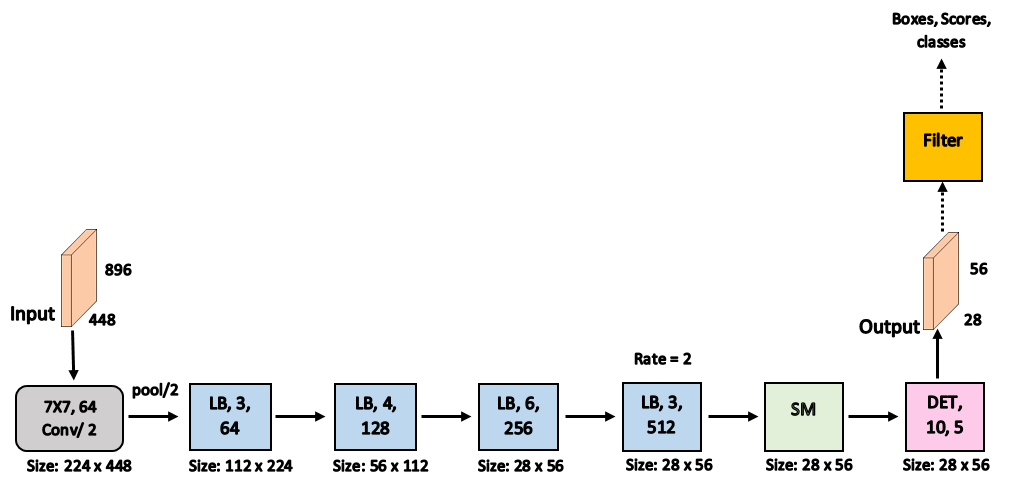
\includegraphics[width=\linewidth]{img/arhitectura_retea.png}
  \caption{Arhitectura re'telei}
  \label{fig:arhitectura_retea}
\end{figure}

Imaginea \ref{fig:arhitectura_retea} ilustreaz'a arhitectura re'telei folosite pentru detec'tia s'age'tilor direc'tionale. Reprezint'a o fuziune 'intre arhitecturile Resnet~\cite{Resnet} 'si YOLO~\cite{YOLO}. Prima este responsabil'a pentru extragerea tr'as'aturilor din imagini, 'in timp ce a doua utilizeaz'a aceste informa'tii 'in predic'tia regiunilor care con'tin s'age'ti. Arhitectura Resnet este aleas'a pentru performan'ta realizat'a at\^at 'in probleme de clasificare, de segmentare c\^at 'si de detec'tie. Arhitectura YOLO este aleas'a pentru timpul de predic'tie redus oferit prin realizarea localiz'arii 'si a clasific'arii prin componenta care extrage tras'aturile din imagini.

Arhitectura este alc'atuit'a din urm'atoarele componente:
\begin{enumerate}
\item Un strat de convolu'tie cu 64 de filtre de 7x7 'si saltul 2. Acesta este urmat de normalizarea pe lot a volumului rezultat 'si aplicarea func'tiei de activare LeakyReLU pe informa'tiile normalizate.
\item Un strat de max pooling care reduce la jum'atate dimensiune h'ar'tii de tr'as'aturi.
\item Patru straturi de blocuri Resnet.
\item O component'a pentru scal'ari multiple ale tr'as'aturilor.
\item O component'a de detec'tie.
\item O component'a pentru filtrarea regiunilor propuse; aceast'a component'a este aplicat'a doar 'in predic'tia re'telei, nu 'si 'in antrenare.
\end{enumerate}

Modelul folosit pentru extragerea tr'as'aturilor este Resnet50. Conform cu acesta, primul strat are 3 blocuri, al doilea 4, al treilea 6 'si al patrulea 3. Parametrii primelor trei componente ale acestei arhitecturi, elementele modelului Resnet50, sunt ini'tializa'ti cu valorile parametrilor antrena'ti pe clasificarea unui alt set de date. Parametrii ini'tializa'ti prin aceast'a tehnic'a se numesc parametrii preantrena'ti 'si produc o 'inv'a'tare mai rapid'a a re'telei. Caracteristic arhitecturii YOLO, predic'tia codific'a informa'tii despre loca'tiile 'si clasele s'age'tilor din imagini. Informa'tiile negative ale predic'tiilor sunt relevante 'in localizarea regiunilor, motiv pentru care func'tia de activare utilizat'a 'in re'tea este LeakyReLU.

'In diagrama conceptual'a sunt precizate dimensiunile datelor de intrare, a celor prezise de re'tea 'si a celor utilizate de componentele re'telei. Imaginile de intrare, cu o rezolu'tie de 1024x2048, sunt redimensionate la 448x896 pentru a corespunde cu dimensiunea a'steptat'a de re'tea. Intr'arile sunt reduse cu un factor de 16, ie'sirile prezise av\^and o rezolu'tie de 28x56. Componentele particip'a sau nu la aceast'a reducerea a intr'arilor, dimensiunile rezultatelor pentru fiecare  component'a fiind specificate sub reprezentarea ei. Se observ'a c'a, un singur strat de pooling este folosit pentru reducerea dimensiunii cu un factor de 2. De restul redimension'arilor se ocup'a straturile de blocuri Resnet 'si convolu'tia cu saltul 2.
 
Definirea arhitecturi este realizat'a prin construirea blocurilor prezente 'in diagrama conceptual'a \ref{fig:arhitectura_retea} utiliz\^and func'tiilor prezente 'in libr'ariile \textit{layers} (tf.layers.conv2d, tf.layers.batch,  tf.layers.max\_pooling2d) 'si \textit{nn} (tf.nn.avg\_pool, tf.nn.atrous\_conv2d, tf.nn.leaky\_relu, tf.nn.softmax) ale framework-ului Tensorflow. Defininea modelului este realizat'a prin func'tia \textit{build(data, training, name, reuse, image\_shape, max\_boxes, score\_threshold, iou\_threshold)}, care conecteaz'a elementele componente conform arhitecturii conceptuale. Parametrii acestei func'tii au urm'atoarea semnifica'tie:
\begin{itemize}
\item data: imaginile de intrare redimensionate la 448x896
\item training: valoarea boolean'a care specific'a dac'a func'tia este apelat'a 'in procesul de antrenare sau 'in cel de evaluare; normalizarea pe lot este aplicat'a diferit 'in cele dou'a etape
\item name: numele modelului; permite partajarea parametrilor 'intre mai multe modele definite cu acela'si nume
\item image\_shape: vector necesar 'in cazul predic'tiei; con'tine dimensiunea imaginii pentru care vor fi realizate predic'tiile
\item max\_boxes: num'arul maxim de regiuni propuse 'intr-o predic'tie; implicit are valoarea 10
\item score\_threshold: scorul de confiden't'a necesar pentru ca o regiune propus'a s'a fie relevant'a; implicit are valoarea 0.5
\item iou\_threshold: valoarea operatorului IOU pentru care suprimarea non-maximelor locale este aplicat'a pe regiunile propuse; implicit are valoarea 0.5
\end{itemize}

\subsection{Componentele arhitecturii}
\subsubsection{Blocul Resnet}
\begin{figure}[H]
  \includegraphics[width=0.7\linewidth]{img/resnet_block.jpg}
  \centering
  \caption{Structura blocului care nu modific'a dimensiunea intr'arii (st\^anga) 'si structura blocului care redimensioneaz'a informa'tiile de intrare prin convolu'tii (dreapta)\protect \footnotemark}
  \label{fig:resnet_block}
\end{figure}
\footnotetext{Imagine adaptat'a din: https://www.researchgate.net/publication/321347448\_Exposing\_Computer\_Genera-ted\_Images\_by\_Using\_Deep\_Convolutional\_Neural\_Networks}

Elementul de baz'a pentru extragerea tr'as'aturilor, ilustrat 'in figura \ref{fig:resnet_block}, 'il constituie blocul rezidual din arhitectura Resnet ~\cite{Resnet}. Este alc'atuit din succesiunea a 3 straturi convolu'tionale cu dimensiunea spa'tial'a a filtrelor de 1x1, 3x3 'si 1x1. Ultimul strat al acestui succesiuni are un num'ar de filtre de patru ori mai mare comparativ cu primele dou'a. Convolu'tiile sunt urmate de normalizarea pe lot a h'ar'tii de tr'as'aturi, informa'tiile normalizate fiind aplicate func'tiei de activare LeakyReLU. 
Ultimul strat de convolu'tie este urmat de normalizarea tr'as'aturilor, 'ins'a func'tia de activare nu este aplicat'a pe aceste informa'tii, ci pe combina'tia acestora cu tr'as'aturile de intrare prin leg'atura de skip connection. 'In re'tea sunt prezente dou'a tipuri de blocuri Resnet: cele care p'astreaz'a dimensiunea de intrare 'si cele care reduc la jum'atate aceast'a dimensiune. 'In imaginea din dreapta a \ref{fig:resnet_block} este prezentat cel de-al doilea bloc. Reduce dimensiunea volumului de intrare la jum'atate prin aplicarea unui salt de 2 'in prima convolu'tie a acestuia. Rezultatul celor trei convolu'tii nu are aceea'si dimensiune cu volumul de intrare al blocului, motiv pentru care aplicarea leg'aturii de skip connection celor dou'a informa'tii nu poate fi realizat'a prin func'tia identitate. 'In cazul acestui bloc leg'atura este realizat'a prin aplicarea unei convolu'tii suplimentare cu salt 2. Comparativ cu blocul Resnet, 'in care este utilizat'a func'tia de activare ReLU, elementul acestei arhitecturi folose'ste LeakyReLU.

Cele descrise mai sus sunt ad'augate 'in modelul re'telei prin func'tia \textit{blockElement(inputs, filters, stride, training, reduceInput, preTrained)}. Parametrii func'tiei sunt urm'atorii:
\begin{itemize}
\item inputs: tr'as'aturile de intrare ale blocului Resnet
\item filters: num'arul de filtre folosit de bloc, indicat prin \textit{f} 'in figura \ref{fig:resnet_block}
\item stride: saltul primei convolu'tii; dac'a acesta este 2 blocul reduce dimensiune intr'arilor
\item training: valoare boolean'a care specific'a dac'a func'tia este apelat'a 'in procesul de antrenare sau 'in cel de evaluare
\item reduceInput: valoare boolean'a care specific'a dac'a leg'atura de skip connection este realizat'a printr-o convolu'tie suplimentar'a
\item preTrained: valoare boolean'a care specific'a dac'a parametrii blocului sunt ini'tializa'ti aleator sau sunt preantrena'ti
\end{itemize}

\subsubsection{Strat de blocuri Resnet}

\begin{figure}[H]
  \includegraphics[width=0.65\linewidth]{img/blocklayer.png}
  \centering
  \caption{Strat Resnet}
  \label{fig:Layer_Resnet}
\end{figure}

Blocurile elementare descrise anterior sunt grupate 'in straturi, dup'a cum este prezentat 'in figura \ref{fig:Layer_Resnet}. Acestea sunt alc'atuite dintr-un num'ar de elemente ale c'aror intr'ari au aceea'si dimensiune spa'tial'a. Primul bloc are structura celui care reduce dimensiunea de intrare, acesta fiind elementul care reduce dimensiunea tr'as'aturilor. 'In figura \ref{fig:arhitectura_retea} se observ'a c'a reducerea volumului de intrare este realizat'a doar de al doilea 'si al treilea strat de blocuri al arhitecturii. Pentru a nu modifica dimensiunea intr'arii, celelalte dou'a straturi nu aplic'a saltul de 2 folosit 'in primul bloc. Structura acestuia nu se modific'a, convolu'tia de 1x1 folosit'a pentru redimensionarea intr'arii fiind folosit'a cu saltul 1. Al patrulea strat al arhitecturii folose'ste convolu'tii atrou cu rata de dilatare 2 'in locul convolu'tiilor obi'snuite de 3x3 din fiecare bloc al acestuia, modalitate prin care tr'as'aturile extrase sunt mai dense, dup'a cum este descris 'in ~\cite{DeepLabV3}.

Func'tia \textit{blockLayer(inputs, filters, strides, blocks, training, name)} este definit'a pentru ad'augarea acestei componente 'in modelul re'telei. Parametrii func'tiei sunt urm'atorii:
\begin{itemize}
\item inputs: tr'as'aturile de intrare ale blocului Resnet
\item filters: num'arul de filtre folosit de blocuri, indicat prin \textit{f} 'in figura \ref{fig:Layer_Resnet}
\item strides: saltul primei convolu'tii; dac'a acesta este 2 blocul reduce dimensiune intr'arilor
\item blocks: num'arul de blocuri ale stratului
\item training: valoare boolean'a care specific'a dac'a func'tia este apelat'a 'in procesul de antrenare sau 'in cel de evaluare
\item name: numele atribuit blocului; este necesar'a denumirea acestora pentru ca evaluarea performan'tei 'in procesul de antrenare s'a fie posibil'a
\end{itemize}

\subsubsection{Component'a pentru multiple scal'ari ale tr'as'aturilor}
Componenta este destinat'a interpret'arii informa'tiilor de intrare la mai multe scale de reprezentare, conform celor prezentate 'in  ~\cite{DeepLabV3}. Captarea contextului global al volumul de intrare este realizat'a prin componenta \ref{fig:image_pooling}. Aceasta este alc'atuit'a dintr-un strat de global average pooling, reprezent\^and cazul extrem al stratului de average pooling 'in care dimensiunea ferestrei este egal'a cu cea a volumului de intrare. Volumul de ie'sire este aplicat unei convolu'tii cu 256 de filtre de 1x1. Rezultatul convolu'tiei este aplicat normaliz'arii pe lot 'si apoi adus la dimensiunea intr'arii prin intermediul interpol'ari biliniare. 

\begin{figure}[H]
  \includegraphics[width=0.9\linewidth]{img/image_pooling.png}
  \centering
  \caption{Image pooling}
  \label{fig:image_pooling}
\end{figure}

Extragerea tr'as'aturilor la multiple dimensiuni este realizat'a prin atrou spatial pyramid pooling, descris 'in subsec'tiunea \ref{ch:aspp}. Alegerea ratelor de dilatare ale celor patru convolu'tii atrou este important'a, prin aceste valori fiind specificat'a m'arimea cu care este extins c\^ampul vizual. Convolu'tiile extind dimensiunea intr'arii cu valori de zero 'in jurul marginilor astfel 'inc\^at dimensiune rezultatului s'a fie egal'a cu cea de intrare, indiferent de rata aplicat'a. Alegerea valorilor mari pentru ratele de dilatare duce la suprapunerea unui num'ar mic de parametrii ai filtrelor peste regiuni de informa'tie. Pentru a permite interpretarea volumului de intrare la multiple dimensiuni, ratele de dilatare sunt alese relativ la dimensiunea acestuia. Pentru dimensiunea spa'tial'a a volumului de intrare (28x56), stratul este alc'atuit din 3 convolu'tii atrou cu 256 de filtre de 3x3 cu rate de dilatare de 4, 8, respectiv 12. Cea de-a patra convolu'tie atrou este 'inlocuit'a cu o convolu'tie obi'snuit'a de 1x1, echivalent'a cu convolu'tia atrou a c'arei rat'a de dilatare corespunde cu dimensiunea volumului de intrare. Rezultatele convolu'tiilor sunt urmate de normalizarea pe lot 'si con'tin tr'as'aturi extrase la dimensiuni diferite de reprezentare. Figura \ref{fig:arrow_aspp} prezint'a structura componentei destinat'a 'inv'a't'arii tr'as'aturilor la multiple dimensiune. Este alc'atuit din cele 4 convolu'tii descrise anterior 'si din componenta care interpretez'a contextul global al volumului de intrare. Rezultatul este compus prin concatenarea celor 5 ie'siri produse de fiecare element 'in parte.

\begin{figure}[H]
  \includegraphics[width=0.9\linewidth]{img/arrow_aspp.png}
  \centering
  \caption{Strat destinat interpret'arii informa'tiilor la multiple scale \protect \footnotemark}
  \label{fig:arrow_aspp}
\end{figure}
\footnotetext{Imagine inspirat'a din: https://ai.googleblog.com/2018/03/semantic-image-segmentation-with.html}

Componenta este ad'augat'a 'in modelul re'telei prin definirea func'tiei \textit{asppLayer(inputs, training, name)}. Parametrii acesteia au aceea'si semnifica'tie cu cei prezenta'ti 'in componenta anterioar'a cu acela'si nume.

\subsubsection{Component'a de detec'tiei}
Componenta destinat'a detec'tiei, ilustrat'a 'in figura \ref{fig:arrow_detection}, utilizeaz'a tr'as'aturile extrase de celelalte componente ale arhitecturii pentru predic'tia regiunilor care con'tin s'age'ti. Componenta este alc'atuit'a din 3 convolu'tii cu filtre de 1x1, 3x3 'si 1x1, asem'an'ator structurii unui bloc Resnet. Convolu'tiile nu modific'a dimensiunea volumului de intrare. Primele dou'a sunt urmate de normalizarea pe lot 'si informa'tiile normalizate sunt aplicate func'tiei de activare LeakyReLU.  Asupra celei de-a treia convolu'tii nu se aplic'a nicio transformat'a, rezultatul acesteia fiind predic'tia re'telei. Primele dou'a convolu'tii au 256, 512 filtre. Num'arul filtrelor 'in ultima convolu'tie este ales pe baza num'arului ancorelor folosite de re'tea 'si de num'arul claselor de interes.

\begin{figure}[H]
  \centering
  \includegraphics[width=1.1\linewidth]{img/arrow_detection.png}
  \centering
  \caption{Strat destinat detec'tiei}
  \label{fig:arrow_detection}
\end{figure}

Este necesar ca num'arul de filtre al ultimei convolu'tii s'a fie egal cu $n * (5 + k)$, unde n este num'arul de ancore 'si k num'arul de clase. Motivarea acestui num'ar este indicat'a de modalitatea prin care predic'tia re'telei codific'a regiunile propuse 'in YOLO. Num'arul canalelor de ad\^ancime ale predic'tiei este egal cu cel al filtrelor aplicate 'in ultima convolu'tie. Conform celor descrise 'in subsec'tiunea \ref{ch:yolo}, fiecare pixel din dimensiunea spa'tial'a propune n regiuni, una pentru fiecare ancor'a. Propunerile sunt realizate pe baza tututor canalelor de ad\^ancime de la pozi'tia spa'tial'a a pixelului, dup'a cum este ilustrat 'in \ref{fig:yolo_detect}.


Coordonatele x 'si y ale predic'tiei trebuie s'a fie valori din intervalul [0,1] pentru a indica pozi'tia 'in interiorul unei celule, scorurile de confiden't'a trebuie s'a corespund'a aceluia'si interval pentru a reprezenta o probabilitate 'si probabilit'a'tile claselor pentru o ancor'a trebuie s'a reprezinte o distribu'tie de probabilitate. Aceste restric'tii sunt 'indeplinite prin aplicarea func'tiei sigmoid'a pentru coordonate 'si scorul de confiden't'a 'si a func'tiei softmax pentru probabilit'a'tile de clase. Rectific'arile acestor valori nu sunt realizate 'in rezultatul acestei componente, deoarece nu toate canalele predic'tiei necesit'a rectific'ari ale valorilor 'si nu toate canalele cu valori condi'tionate utilizeaz'a aceea'si func'tie de activare. 

\begin{figure}[H]
  \centering
  \includegraphics[width=1.1\linewidth]{img/yolo_detect.png}
  \caption{Codificarea predic'tiei 'in YOLO \protect \footnotemark}
  \label{fig:yolo_detect}
\end{figure}
\footnotetext{Imagine inspirat'a din: https://cdn-images-1.medium.com/max/1600/1*d\_Yv2xJSoscLoX8twmaAmQ.png}

Componenta este ad'augat'a 'in modelul re'telei prin definirea func'tiei \textit{detectLayer(inputs, training, nrAnchors, nrClasses)}. Parametrul \textit{nrAnchors} specific'a num'arul ancorelor folosite de re'tea 'si \textit{nrClasses} specific'a num'arul claselor de interes. Dup'a cum a fost descris, pe baza acestor parametrii este ales num'arul de filtre al ultimei convolu'tii.

\subsubsection{Component'a pentru filtrare}
Componenta este aplicat'a doar 'in procesul de evaluare 'si cel de testare. Constituie etapa de postprocesare a regiunilor propuse fiind realizat'a prin eliminarea regiunilor cu produsul dintre scorul de confiden't'a 'si probabilitatea unei clasei mai mic dec\^at un prag ales. Tehnica de suprimare a non-maximelor locale este aplicat'a pe regiunile alese 'in urma filtr'arii pentru a elimina predic'tiile redundante ale unei s'age'ti. Componenta este ad'augat'a 'in modelul re'telei prin definirea func'tiei \textit{non\_maximum\_suppresion(output, image\_shape, max\_boxes, score\_threshold, iou\_threshold)}. Rectific'a valorile predic'tiei prin func'tia sigmoid'a 'si softmax pe canalele necesare. Parametrul \textit{output} reprezint'a predic'tia re'telei, restul parametrilor av\^and aceea'si semnifica'tie cu cei din func'tia \textit{build} cu acela'si nume.

\subsection{Optimizarea re'telei}
\subsubsection{Func'tia de cost}
Re'teaua descris'a anterior realizeaz'a at\^at localizarea c\^at 'si clasificarea s'age'tilor prin propunerea de regiuni. Func'tia de cost a acesteia trebuie s'a minimizeze erorile ambelor probleme, trat\^and simultan erorile de clasificare a regiunilor de interes 'si coordonatele acestora. Func'tia de cost aplicat'a este cea folosit'a 'in arhitectura YOLO~\cite{YOLO} 'si descris'a 'in subsec'tiunea \ref{ch:yolo}.

\begin{equation}
\begin{split}
L(\theta) = & \lambda_{coord} * \sum\limits_{i=0}^{m_w*m_h} \sum\limits_{j=0}^{B} gt_{ij}^{dim} * 1_{ij}^{obj}[(x_i - \hat{x}_i)^2 + (y_i - \hat{y}_i)^2 + (w_i - \hat{w}_i)^2 + (h_i - \hat{h}_i)^2] \\
& + \sum\limits_{i=0}^{m_w*m_h} \sum\limits_{j=0}^{B} 1_{ij}^{obj}(C_i - \hat{C}_i)^2\\
& + \lambda_{nocoord} \sum\limits_{i=0}^{m_w*m_h} \sum\limits_{j=0}^{B} 1_{ij}^{noobj}(C_i - \hat{C}_i)^2 \\
& + \sum\limits_{i=0}^{m_w*m_h} 1_{ij}^{obj} \sum\limits_{c \in classes} (p_i(c) - \hat{p}_i(c))^2
\end{split}
\label{eq:yolo2}
\end{equation}

Ecua'tia \ref{eq:yolo2} prezint'a metrica folosit'a pentru calcularea similarit'a'tii dintre regiunile propuse 'si cele de ground truth.  M'a'stile 'si parametrii necesari func'tiei de cost YOLO sunt descri'si 'in subsec'tiunea \ref{ch:yolo}. Comparativ cu aceast'a func'tie, cea ilustrat'a 'in  ecua'tia \ref{eq:yolo2} folose'ste o masc'a suplimentar'a, \textit{$gt_{ij}^{dim}$}. Masca este definit'a pe baza m'arimii regiunii de ground truth 'si const'a 'in asigurarea unei invarian'te a erorii de localizare la dimensiunea regiunilor de ground truth. Consider\^and $g_w$ 'si $g_h$ lungimea 'si 'in'al'timea normalizat'a a unei astfel de regiuni, prezis'a de zona construit'a pe baza celulei i 'si a ancorei j, valoarea m'a'stii este definit'a prin: $gt_{ij}^{dim} = 1 - g_w * g_h$. Aplicarea acestei func'tii de cost trebuie s'a tin'a cont de mai multe aspecte: eroarea de localizarea trebuie realizat'a pe coordonate reprezentate 'in formatul codificat al re'telei, scorul de confiden't'a pentru o regiune de fundal este 0 'si pentru o regiune de interes are valoarea maxim'a ob'tinut'a prin suprapunerea regiunilor de ground truth cu predic'tiile corespunz'atoare prin pozi'tie. Urm'atorul pseudocod ilustreaz'a modul de calculare al func'tiei de cost pe baza acestor aspecte.

\begin{algorithmic}
\Require $rezultat, ground\_truth, ancore, 1^{obj}, delta\_box, gt^{dim}$
\Ensure cost\_total
\State $xywh, conf, cls \Leftarrow decode(rezultat)$\Comment{Decodificarea predic'tiei}
\State $box \Leftarrow construct(xywh, ancore)$\Comment{Contruc'tia regiunilor propuse}
\State $scor\_iou \Leftarrow iou\_op(ground\_truth, box)$
\Comment{IOU pe fiecare regiune real'a 'si propus'a}
\State $obj\_det \Leftarrow scor\_iou > 0.6$ 
\State $no\_obj \Leftarrow (1 - obj\_det) * (1 - 1^{obj})$ \Comment{$no\_obj$ este $1^{noobj}$}
\State $no\_obj\_loss \Leftarrow \lambda_{nocoord} * no\_obj * (- conf) ^ 2$ \Comment{$c_i$ este 0 pentru fundal}
\State $obj\_loss \Leftarrow \lambda_{coord} * 1^{obj} * (scor\_iou - conf) ^ 2$ \Comment{$c_i$ este valoarea iou cea mai mare}
\State $cost\_conf \Leftarrow obj\_loss + no\_obj\_loss$
\State $cost\_cls \Leftarrow 1^{obj} * (delta\_box[4] - cls) ^ 2$
\State $cost\_coord \Leftarrow \lambda_{coord} * 1^{obj} * gt^{dim} * (delta\_box[0:4] - xywh) ^ 2$
\State $cost\_total \Leftarrow cost\_conf + cost\_cls + cost\_coord$
\end{algorithmic}

\leavevmode \newline
Calcularea func'tiei de cost este realizat'a de metoda \textit{computeLoss(output, ground\_truth\_boxes, selected\_box\_mask, selected\_delta\_boxes, scale\_by\_dimensions)}. Parametrii func'tiei indic'a:
\begin{itemize}
\item output: predic'tia re'telei
\item ground\_truth\_boxes: regiunile de ground truth ale predic'tiei
\item selected\_box\_mask: masc'a care specific'a dac'a o regiune prezis'a corespunde cu o regiune de ground truth; coresponden'ta este realizat'a pe baza pozi'tiei regiunii de ground truth 'in dimensiunea spa'tial'a a predic'tiilor
\item selected\_delta\_boxes: masc'a care con'tine regiunile de ground truth 'in formatul codificat al  predic'tiilor 
\item scale\_by\_dimensions: masc'a care asigur'a invarian'ta la dimensiunile regiunilor ($gt_{ij}^{dim}$)
\end{itemize}

\subsubsection{Regularizarea L2}
'In capitolul anterior a fost specificat'a importan'ta regulariz'arii 'in re'teaua de fa't'a. Dup'a cum a fost precizat, asigur'a stabilitatea acesteia 'si o generalizare bazat'a pe tr'as'aturile esen'tiale ale s'age'tilor. Parametrul care penalizeaz'a parametrii cu valori mari este $\lambda = 0.00005$. Valoarea acestuia este mic'a, deoarece fiecare component'a a re'telei aplic'a normalizarea pe lot asupra h'ar'tii de tr'as'aturi. 

Regularizarea este aplicat'a asupra filtrelor din straturile convolu'tionale ale re'telei. Introducerea tehnicii 'in modelul re'telei este realizat'a prin func'tia \textit{tf.layers.conv2d}, func'tie utilizat'a la fiecare definire a unui strat convolu'tional. Parametrul \textit{kernel\_regularizer} al acestei func'tii specific'a tehnica de regularizare aplicat'a pe filtrele convolu'tionale. Ad'augarea regularizatorului L2 const'a 'in atribuirea func'tiei \textit{ tf.contrib.layers.l2\_regularizer(scale = 5e-4)} acestui parametru.

\subsubsection{Adam}
Unul dintre cele mai importante elemente ale procesului de 'inv'a'tare 'il constituie optimizatorul folosit. Re'teaua propus'a utilizeaz'a Adam datorit'a avantajelor sale descrise 'in partea teoretic'a: eliminarea zgomotului din tr'as'aturile 'inv'a'tate 'si a problemei de vanishing gradient. Integrarea acestuia 'in modelul re'telei este efectuat'a prin instan'tierea unei clase \textit{tf.train.AdamOptimizer}. Pentru crearea sa trebuie specificat'a rata de 'inv'a'tare folosit'a (0.0001). Minimizarea func'tiei de cost pe baza optimizatorului este realizat'a prin func'tia \textit{minimize(loss, global\_step)} din clasa instan'tiat'a. Parametrii acestei func'tii au urm'atoarea semnifica'tie:
\begin{itemize}
\item loss: func'tia de cost a pasului curent
\item global\_step: num'arul pasului curent
\end{itemize}

\section{Etape de preprocesare}
\subsection{Selec'tia ancorelor}
Ancorele folosite pentru realizarea predic'tiilor sunt selectate 'intr-o etap'a de preprocesare pe baza metodei de grupara K-means, descris'a 'in sec'tiunea \ref{ch:k-means}. Scopul urm'arit este identificarea celor mai comune dimensiuni ale regiunilor care con'tin s'age'ti direc'tionale 'in imagini. Vectorul de tr'as'aturi utilizat pentru partajarea dimensiunilor con'tine dou'a elemente: lungimea 'si in'al'timea regiunii reale. K-means este aplicat pe vectorii de tr'as'aturi ale regiunilor care con'tin s'age'ti din setul de antrenare. M'asurarea similarit'a'tii dintre doi vectori de tr'as'aturi prin distan'ta euclidian'a, are erori mai mari pentru regiunile mari comparativ cu cele mici. Efectul produs de utilizarea acestei distan'te este cel de favorizare al regiunilor mici. O distan'ta independent'a de dimensiunea regiunilor este bazat'a pe operatorul IOU pentru m'asurarea similarit'a'tii dintre doi vectori de tr'as'aturi, distan'ta fiind definit'a 'in acest caz prin ecua'tia \ref{eq:dist_iou}, unde \textit{x} este un vector de tr'as'aturi 'si $c_i$ centrul curent al grupului i.

\begin{equation}
d(x, c_i) = 1 - IOU(x, c_i)
\label{eq:dist_iou}
\end{equation}

Tehnica de grupare a regiunilor pe baza dimensiunii este efectuat'a prin aplicarea clasei \textit{KMeans} pe toate regiunile setului de date. A fost necesar'a definirea unei clase proprii, deoarece implement'arile existente 'in python nu permit modificarea distan'tei euclidiene folosite. La instan'tierea clasei este specificat'a calea absolut'a a directorului care con'tine regiunile setului de antrenare. Acestea sunt desprinse din fi'sierele xml de ground-truth, motiv pentru care acest director trebuie s'a indice calea c'atre fi'sierele xml. 

Aplicarea grup'arii K-means folosind clasa definit'a este realizat'a prin apelul func'tiei \textit{run(iterations, k, dims)}. Parametrii acesteia sunt urm'atorii:
\begin{itemize}
\item iterations: num'arul maxim al itera'tiilor aplicate 'in parti'tionarea regiunilor 'in grupuri
\item k: num'arul de grupuri; implicit are valoarea 10
\item dims: dimensiunea pe care ancorele vor fi aplicate (predic'tia re'telei); implicit are valoarea [28,56]
\end{itemize}
 
\subsection{Calcularea m'a'stilor func'tiei de cost}
Fiecare regiune de ground truth este asociat'a cu o regiune propus'a pe baza dimensiunii acesteia 'si a loca'tiei sale 'in imagine. Calcularea m'a'stilor pe baza informa'tiilor din regiunile reale determin'a penalizarea regiunilor propuse care corespund prin loca'tie, 'in predic'tia re'telei, cu acele informa'tii de ground truth. Corespunden'ta dintre o regiune a'steptat'a 'si o regiune propus'a este realizat'a conform cu urm'atorul pseudocod:
\newpage
\begin{algorithmic}
\Require $ancore, ground\_truth$
\Ensure i, j, index\_ancora \Comment{Pozi'tia 'si ancora unui regiuni reale}
\State $box \Leftarrow ground\_truth * (W, H, W, H)$\Comment{Redimensionarea la dimensiunea predic'tiei}
\State $i \Leftarrow int(box.y)$
\State $j \Leftarrow int(box.x)$
\State $index\_ancora \Leftarrow 0$
\State $best\_iou \Leftarrow 0$
\For{$k \gets 1, nr\_ancore$}
\State $a \Leftarrow ancore[k]$
\State $iou \Leftarrow iou\_op(a, box)$ \Comment{iou\_op este operatorul IOU}
\If{$iou > best\_iou$}
  \State $best\_iou\Leftarrow iou$
  \State $index\_ancora \Leftarrow k$
\EndIf
\EndFor
\end{algorithmic}

\leavevmode \newline
M'a'stile utilizare 'in func'tia de cost sunt calculate conform cu pozi'tiile 'si ancorele corespondente regiunile de ground truth:
\begin{itemize}
\item \textbf{selected\_box\_mask} ($1^{obj}$):  Masca specific'a dac'a o regiune prezis'a corespunde cu o regiune de ground truth. Valorile din masc'a corespunz'atoare pozi'tiilor 'si ancorelor sunt 1, restul elementelor fiind 0. 
 
\item \textbf{selected\_delta\_boxes}: Masca con'tine coordonatele 'si clasele regiunilor de ground truth 'in formatul codificat al predic'tiilor.  Valorile din masc'a corespunz'atoare pozi'tiilor 'si ancorelor sunt codificate conform ecua'tiilor \ref{eq:cod}, restul elementelor fiind 0. Pentru un anumit ground truth \textit{b} cu pozi'tia \textit{(i,j)} 'si ancora \textit{a} masca va con'tine urm'atoarele valori:
\begin{equation}
\begin{split}
x = b.x - j \\
y = b.y - i \\
w = \log(b.w / a.w) \\
h = \log(b.h / a.h) \\
\end{split}
\label{eq:cod}
\end{equation}

\item \textbf{scale\_by\_dimensions} ($gt^{dim}$): Masca con'tine factorul de scalare al erorii de localizare pe baza m'arimii regiuniilor de ground truth. Valorile din masc'a corespunz'atoare pozi'tiilor 'si ancorelor sunt calculate conform m'arimii regiunilor, restul elementelor fiind 0.
\end{itemize}

\section{'Imbun'at'a'tirea performan'tei}
\subsection{Reducerea num'arului de filtre}
Reducerea num'arului de filtre nu este destinat'a cre'sterii performan'tei, ci a altul aspect important al re'telei: timpul de inferen't'a. Reducerea dimensiunii poate fi realizat'a prin reducerea num'arului de filtre sau a celui de blocuri Resnet aplicate 'in fiecare strat de blocuri. Prima solu'tie reduce num'arul tr'as'aturilor esen'tiale identificate de re'tea, 'in timp ce a doua abordare reduce complexitatea pe care o poate 'inv'a'ta re'teaua. 'Intruc\^at num'arul de clase de interes este mic 'si varia'tiile 'in reprezentarea unui obiect sunt influen'tate doar de proiec'tia 'in imagine, prima solu'tie este cea aleas'a. Pentru a implementa aceast'a modificare 'in modelul descris este necesar'a ad'augarea unui parametru nou 'in func'tia care contruie'ste modelul re'telei, \textit{nr\_filters}. Acesta specific'a num'arul de filtre al primului strat de blocuri Resnet, restul fiind calculate pe baza acestuia prin: $nr\_filters * (2^i)$, unde i reprezint'a deplasamentul fa't'a de primul strat.

\subsection{Normalizarea pe grup}
Sistemul de fa't'a 'inva't'a detec'tia s'age'tilor direc'tionale prin intermediul imaginilor de rezolu'tie mare. Dimensiunea imaginilor reduce num'arul de loturi ce pot fi 'inv'a'tate 'in paralel, motiv pentru care normalizarea pe lot poate limita performan'ta sistemului. Chiar dac'a num'arul de instan'te antrenate 'in paralel este redus, num'arul regiunilor de interes este mai mare, deoarece o imagine poate con'tine mai multe s'age'ti. Normalizarea pe grup, prezentat'a 'in capitolul anterior, poate 'imbun'at'a'ti performan'ta sistemului 'in cazul 'in care normalizarea pe lot limiteaz'a aceast'a valoare. Noua tehnic'a de normalizare a fost inclus'a 'in modelul re'telei prin 'imp'ar'tirea canalelor din volumul de intrare al fiec'arui strat 'in grupuri de 32, media 'si varia'tia fiind calculate pe aceste grupuri. Integrarea acestei tehnici 'in modelul re'telei nu a ajutat la cre'sterea performan'tei, deoarece parametrii preantrena'ti utiliza'ti pentru extragerea tr'as'aturilor au fost determina'ti prin normalizarea pe lot. Aceast'a normalizare necesit'a ini'tializarea aleatoare a tuturor parametrilor, motiv pentru care nu va mai fi utilizat'a 'in solu'tia final'a a modelului.

\subsection{Rata de 'inv'a'tare ciclic'a}
O 'imbun'at'a'tire a performan'tei poate fi realizat'a prin introducerea unei rate de 'inv'a'tare ciclice, dup'a cum a fost prezentat 'in capitolul anterior. Aplicarea acesteia 'impreun'a cu optimizatorul Adam presupune modificarea valorii ratei de 'inv'a'tare folosit'a 'in fiecare pas al procesului de antrenare. Modificarea ratei de 'inv'a'tare prin politica "triunghi", politic'a descris'a 'in capitolul anterior, nu a ajutat la cre'sterea performan'tei 'in detec'tie. Acest lucru poate fi datorat unei alegeri nepotrivite a parametrilor folosi'ti 'in aplicarea tehnicii. Limita inferioar'a 'si cea exterioar'a sunt experimental u'sor de identificat, 'ins'a num'arul de itera'tii 'in care se ajunge de la o limit'a la alta este mai dificil de identificat. Pentru a observa dac'a o alegere necorespunz'atoare a acestui parametru au influen'tat performan'ta re'telei, o nou'a politic'a a fost aplicat'a 'in modelul re'telei, politic'a descris'a 'in~\cite{clr_cos}. Aceasta se bazeaz'a pe func'tia de cosinus 'si reseteaz'a la maxim valoarea ratei de 'inv'a'tare c\^and minimul este atins (un ciclu de actualizare al ratei este complet). Aplicarea acesteia 'impreun'a cu optimizatorul Adam au ajutat la 'imbun'at'a'tirea performan'tei. Comparativ cu politica "triunghi", aceast'a tehnic'a doar descre'ste valoarea ratei de 'inv'a'tare de-a lungul unui ciclu.

\begin{figure}[H]
  \centering
  \includegraphics[width=0.8\linewidth]{img/clr_show.png}
  \caption{Politica ratei de 'inv'a'tare}
  \label{fig:clr_cosinus}
\end{figure}

'In figura \ref{fig:clr_cosinus} este ilustrat'a valoarea ratei de 'inv'a'tare prin politica aplicat'a 'in modelul re'telei. Valoarea maxim'a a tehnicii este aleas'a prin identificarea valorii maxime pentru care optimizatorul Adam converge, 'in cazul de fa't'a 0.0001. Valoarea minim'a trebuie s'a corespund'a cu o valoarea pentru care re'teaua converge, 'in cazul de fa't'a 0.00001. Ciclurile ratei de 'inv'a'tare nu sunt identice, num'arul de pa'si necesari pentru atingerea valorii minime cresc\^and de la un ciclu la altul: primul ciclu atinge maximul dup'a dou'a itera'tii complete peste setul de date, al doilea ciclu dup'a patru, al treilea ciclu dup'a opt 'si a'sa mai departe. 'In figura \ref{fig:implementare} este prezentat'a func'tia care realizeaz'a modificarea ratei de 'inv'a'tare.

\begin{figure}[H]
  \centering
  \includegraphics[width=0.9\linewidth]{img/clr_code.png}
  \caption{Implementarea ratei de 'inv'a'tare ciclice}
  \label{fig:implementare}
\end{figure}

\chapter{Testare 'si Validare}
\section{Performan'ta sistemului}
Evaluarea performan'tei este m'asurat'a prin intermediul metricii mean average precision descris'a 'in \ref{ch:map}. Metrica mAP@0.5 consider'a c'a o regiune propus'a este asociat'a unui ground truth dac'a intersec'tia lor prin operatorul IOU este mai mare dec\^at 0.5. Aplic\^and aceast'a metric'a, evaluarea sistemului poate fi realizat'a dup'a ce procesul de antrenare a fost finalizat, pentru a observa performan'ta acestuia 'in detec'tie. De asemenea, aceast'a metric'a este utilizat'a pentru evaluarea periodic'a a performan'tei modelului 'in timpul procesului de antrenare. Evaluarea const'a 'in aplicarea metricii pe setul de antrenare 'si pe cel de validare 'in anumi'ti pa'si ai procesului de 'inv'a'tare. Aceast'a tehnic'a este utilizat'a pentru a observa modul 'in care re'teaua se comport'a pe un set diferit dec\^at cel observat 'in antrenare, fiind util'a pentru detec'tia overfitting-ului. 'In imaginea \ref{fig:map_retea} este ilustrat'a performan'ta pe setul de antrenare 'si cel de validare 'in timpul 'inv'a'tarii. Se observ'a o cre'stere progresiv'a pe ambele curbe, motiv pentru care putem spune c'a re'teaua nu face overfitting pe s'age'tile din setul de antrenare.

\begin{figure}[H]
\center
\includegraphics[width=0.5\linewidth]{img/map.png}
\caption{mAP@0.5 pe setul de antrenare (portocaliu) 'si cel de validare (albastru)}
\label{fig:map_retea}
\end{figure}

\section{Compara'tii 'intre diferite abord'ari realizate}
\begin{table}[ht]
\centering   
\begin{tabular}{|p{6cm}||p{3cm}|p{3cm}|}
 \hline
 Modelul re'telei & mAP@0.5 & FPS\\
 \hline
 YOLO & 0.65 & 30\\
 RESNET50+YOLO & 0.68 & 15\\
 RESNET50/2+YOLO & 0.63 & 29\\
 RESNET50/2+YOLO+CLR & 0.7 & 29\\
 \hline
\end{tabular}
\caption{Metrica de evaluare 'si fps pentru arhitecturi diferite}
\label{table:nonlin} 
\end{table}

'In tabelul de mai sus sunt prezenta'ti indicatori pentru performan'ta (mAP@0.5) 'si viteza (FPS) diferitelor abord'ari arhitecturale ale sistemului de detec'tie. \textit{RESNET50+YOLO} reprezint'a re'teaua ini'tial'a, care const'a 'in combinarea re'telelor Resnet 'si YOLO. \textit{RESNET50/2} \textit{+YOLO} reprezint'a re'teaua ob'tinut'a dup'a eliminarea a jum'atate din filtrele folosite de Resnet50 din arhitectura ini'tial'a. \textit{RESNET50/2+YOLO+CLR} nu aduce modific'ari arhitecturii re'telei anterioare, 'ins'a adaug'a tehnica ratei de 'inv'a'tare ciclice asupra optimizatorului Adam. Se observ'a impactul adus de reducerea dimensiunii re'telei (cre'ste num'arul imaginilor prezice pe secund'a) 'si a ratei de 'inv'a'tare ciclice (cre'ste performan'ta re'telei). 

Primul model arhitectural este prezentat pentru compararea solu'tiile propuse cu acest modelul destinat detec'tiei. Arhitectura YOLO are un timp de inferen't'a mai redus dec\^at cel al solu'tiilor propuse. Metrica utilizat'a pentru evaluarea performan'tei indic'a o valoare mai sc'azut'a a acestui model comparativ cu modelul final al arhitecturii, chiar dac'a acest model are un num'ar mai redus de parametrii. Ceea ce metrica nu prezint'a este situa'tia pe care modelul YOLO nu o poate generaliza: predic'tia s'age'tilor aflate la distan'te mari. Toate solu'tiile propuse ilustrate 'in tabel permit 'inv'a'tarea tr'as'aturilor la multiple dimensiuni de reprezentare 'si predic'tia s'age'tilor situate la p\^an'a 40m. YOLO 'inv'a'ta tr'as'aturi la o singur'a scal'a de reprezentare, motiv pentru care cele mai comune dimensiuni pentru reprezentarea s'age'tilor sunt re'tinute pentru minimizarea func'tiei de cost.

\section{Rezultate}
'In aceast'a sec'tiune vor fi prezentate rezultate ale sistemului de detec'tie. Acestea sunt constituite din imagini augmentate cu regiunile prezise suprapuse peste imaginnile de intrare. Fiecare regiune din imaginea augmentat'a este colorat'a conform clasei prezise, 'in felul urm'ator: regiunile albastre corespund predic'tiilor pentru s'ageata fa't'a, regiunile verzi corespund predic'tiilor pentru s'ageata st\^anga, regiunile albastre corespund predic'tiilor pentru s'ageata dreapt'a, regiunile albastre corespund predic'tiilor pentru s'ageata fa't'a-st\^anga, regiunile albastre corespund predic'tiilor pentru s'ageata fa't'a-dreapta. Fiecare regiune din imaginea augmentat'a prezint'a scorul de confident'a al re'telei asupra regiunii propuse.

\begin{figure}[H]
  \centering
  \includegraphics[width=\linewidth]{img/result/bielefeld_000000_015587_leftImg8bit.png}
  \caption{Predic'tii cu scor de confiden't'a mare datorat dimensiunii 'si clarit'a'tii s'age'tilor}
\end{figure}

\begin{figure}[H]
  \centering
  \includegraphics[width=\linewidth]{img/result/berlin_000536_000019_leftImg8bit_f.jpg}
    \caption{Predic'tii cu scor de confiden't'a mare datorat dimensiunii 'si clarit'a'tii s'age'tilor}
\end{figure}

\begin{figure}[H]
  \centering
  \includegraphics[width=\linewidth]{img/result/mainz_000003_010880_leftImg8bit_f.jpg}
   \caption{Predic'tii cu scor de confiden't'a mare datorat dimensiunii 'si clarit'a'tii s'age'tilor}
\end{figure}

\begin{figure}[H]
  \centering
  \includegraphics[width=\linewidth]{img/result/bonn_000033_000019_leftImg8bit.png}
  \caption{Predic'tie cu scor de confiden't'a mai redus datorat deform'arii produse de denivelarea drumului}
\end{figure}

\begin{figure}[H]
  \centering
  \includegraphics[width=\linewidth]{img/result/mainz_000001_035963_leftImg8bit.png}
  \caption{Predic'tii pentru s'age'ti par'tial 'sterse. Scorul de confiden't'a este mai redus pentru s'ageata fa't'a-dreapta par'tial 'stears'a pe direc'tia de orientare.}
\end{figure}

\begin{figure}[H]
  \centering
  \includegraphics[width=\linewidth]{img/result/mainz_000000_000093_leftImg8bit.png}
  \caption{Predic'tii pentru s'age'ti dep'artate. Scorul de confiden't'a este mai redus comparativ cu cel al s'age'tilor aflate 'in aproprierea ma'sinii.}
\end{figure}


\begin{figure}[H]
  \centering
  \includegraphics[width=\linewidth]{img/result/leverkusen_000001_000019_leftImg8bit.png}
  \caption{Predic'tii pentru s'age'ti dep'artate. Scorul de confiden't'a este mai redus comparativ cu cel al s'age'tilor aflate 'in aproprierea ma'sinii.}
\end{figure}

\begin{figure}[H]
  \centering
  \includegraphics[width=\linewidth]{img/result/bielefeld_000000_061975_leftImg8bit_f.jpg}
   \caption{Predic'tii cu scor de confiden't'a mai redus pentru s'ageata par'tial 'stears'a 'si pentru s'age'tile dep'artate.}
\end{figure}

\begin{figure}[H]
  \centering
  \includegraphics[width=\linewidth]{img/result/mainz_000001_016391_leftImg8bit_f.jpg}
  \caption{Predic'tii la multiple distan'te fa't'a de ma'sin'a. Scorul de confiden't'a al regiunilor apropriate este mai mare dec\^at cel al regiunilor situate departe.}
\end{figure}

\begin{figure}[H]
  \centering
  \includegraphics[width=\linewidth]{img/result/munich_000283_000019_leftImg8bit_f.jpg}
   \caption{Predic'tii la multiple distan'te fa't'a de ma'sin'a. Scorul de confiden't'a al regiunilor apropriate este mai mare dec\^at cel al regiunilor situate departe.}
\end{figure}


\chapter{Manual de Instalare 'si Utilizare}
Acest capitol con'tine o descriere a modalit'a'tii de instalare a resursele software necesare pentru utilizarea sistemului de detec'tie. Minimul necesar pentru folosirea acestui sistem 'il constituie utilizarea unui calculator cu sistemul de instalare Windows. Framework-ul 'si libr'ariile utilizate de sistemul re'telei sunt detaliate 'in \ref{ch:install} 'si utilizate pe Windows, motiv pentru care nu este garantat'a execu'tia corect'a pe un alt sistem de operare. Rularea poate fi realizat'a pe CPU sau pe GPU, 'ins'a cea de-a doua  alegere necesit'a instalarea unor resurse software suplimentare, dup'a cum este prezentat \ref{ch:install}.

\section{Instalarea resurselor software necesare}
\label{ch:install}
Instalarea resurselor software necesare pentru antrenarea 'si predic'tia re'telei sunt descrise 'in urm'atorii pa'si:

\begin{enumerate}
\item Instalarea Anaconda folosind urm'atorul link \url{https://www.anaconda.com/download/} prin selectarea versiunii de Windows pe 64 bi'ti compatibil'a cu versiunea de Python 3.5.
Anaconda ofer'a o modalitate simpl'a de creare a unui mediu virtual 'in care s'a fie instalat 'si folosit framework-ul Tensorflow.
\item Crearea unui nou mediu virtual. Fiecare mediu creat prin Anaconda va avea un nume unic 'si va fi indendent de restul mediilor existente. Un mediu nou este realizat prin deschiderea unui command prompt de Anaconda 'si introducerea comenzii \textit{conda create -n nume\_mediu pip python=3.5} 'inlocuind \textit{nume\_mediu} cu numele dorit.
\item Activarea mediului virtual creat prin introducerea comenzii: \textit{activate nume\_mediu}.
\item Instalarea framework-ului Tensorflow 'in mediul activat. Acesta are disponibile versiuni pentru CPU 'si pentru GPU, prin urm'atoarele comenzi fiind instalat'a versiunea corespunz'atoare resurselor hardware ale calculatorului folosit:
\begin{itemize}
\item Pentru versiunea pe CPU instalarea este realizat'a prin introducerea comenzii: \textit{pip install --ignore-installed --upgrade tensorflow}.
\item Pentru versiunea pe GPU instalarea este realizat'a prin introducerea comenzii: \textit{pip install --ignore-installed --upgrade tensorflow-gpu}.
\end{itemize}
\item Instalarea versiunii de GPU pentru Tensorflow necesit'a instalarea suplimentar'a a urm'atoarelor resurse:
\begin{itemize}
\item CUDA® Toolkit 9.0. Pentru mai multe detalii, consulta'ti documenta'tia NVIDIA: \url{https://docs.nvidia.com/cuda/cuda-installation-guide-microsoft-windows/}.\\Ad'auga'ti calea c'atre CUDA la variabila de mediu \%PATH\%.
\item Driverul NVIDIA asociat cu toolkit-ul CUDA.
\item cuDNN v7.0. Ad'auga'ti directorul 'in care a'ti instalat DLL cuDNN 'in variabila de mediu \%PATH\%.
\end{itemize}
\item Sistemul pentru detec'tia s'age'tilor necesit'a libr'arii de Python suplimentare celor incluse la instalarea distribu'tiei Anaconda. Ad'augarea lor 'intr-un anumit mediul virtual este realizat'a prin introducerea comenzii: \textit{pip install nume\_libr'arie}, unde \textit{nume\_libr'arie} reprezint'a libr'aria necesar a fi introdus'a 'in mediul virtual. Aceste comenzi trebuie introduse dup'a ce mediul a fost activat (pasul 3), pentru sistemul de fa't'a fiind necesare urm'atoarele comenzi:
\begin{itemize}
\item Pentru Numpy: \textit{pip install numpy}
\item Pentru OpenCV: \textit{pip install pip
 install opencv-python}
\item Pentru Tensorboard: \textit{pip install tensorboard}. Acest'a aplica'tie este necesar'a pentru vizualiz'ari despre evolu'tia procesului de antrenare 'si performan'ta sistemului.
\end{itemize}
\item Evaluarea performan'tei este realizat'a prin intermediul unui API oferit de Tensorflow. Dac'a dori'ti s'a realiza'ti aceast'a ac'tiune asupra modelului antrenat, este necesar'a ad'augarea API-ului 'in sistemul destinat detec'tie. Pa'sii necesari pentru realizarea acestei opera'tii sunt prezenta'ti 'in: \url{https://github.com/EdjeElectronics/Tensor-} \url{Flow-Object-Detection-API-Tutorial-Train-Multiple-Objects-Windows-10#2-set-up-tensorflow-directory-and-anaconda-virtual-environment}. Pentru integrarea evaluatorului trebuie realiza'ti pa'sii 2d-2f din tutorial.
\end{enumerate}

\section{Utilizarea sistemului} 
\subsection{Predic'tie}
\subsection{Antrenare}
 
 
\chapter{Concluzii}
\section{Contribu'tia 'in domeniu}
\section{Rezultate ob'tinute}
\section{Dezvolt'ari ulterioare}
\subsection{Extidenderea setului de date}
Performan'ta sistemului de detec'tie poate fi 'imbun'at'a'tit'a prin mai multe modalit'a'ti. Un set de date mai mare 'si cu un context mai extins asupra domeniului ajut'a la o generalizarea mai bun'a a sistemului. 

\subsection{'Imbun'at'a'tirea performan'tei}
\subsection{Compresia re'telei}
'In solu'tia propus'a num'arul de filtre al re'telei destinat'a extragerii de tr'as'aturi este redus la jum'atate prin simpla eliminare a acestora. O performan't'a mai bun'a poate fi atins'a prin aplicarea unei metode de compresie re'telei.

%\addcontentsline {toc}{chapter}{Bibliography} 
\bibliographystyle{IEEEtran} 
\bibliography{thesis}%same file name as for .bib

\include{apendix}

\end{document}
